%!TEX root = ../thesis.tex
%*******************************************************************************
%****************************** Fourth Chapter **********************************
%*******************************************************************************
\chapter{MOFs: Metal organic frameworks for drug delivery} \label{chap:MOF}

% Don't forget to PEE/L

% **************************** Define Graphics Path **************************
\ifpdf
    \graphicspath{{Chapter4/Figs/Raster/}{Chapter4/Figs/PDF/}{Chapter4/Figs/}}
\else
    \graphicspath{{Chapter4/Figs/Vector/}{Chapter4/Figs/}}
\fi

``One of the most exciting developments in recent porous-materials science''

\textit{Teplensky et. al, JACS 2017}~\cite{teplensky2017temperature}

\section{Introduction} \label{sec:MOF-intro}
\subsection{siRNA as a cancer treatment}
When the latest statistics find that over half of people born in the UK since 1960 will develop some form of cancer in their lifetime~\cite{ahmad2015trends}, it hardly needs stating that cancer has affected almost everyone in the country in some way. 
Any successful efforts to discover new treatments for this set of diseases are therefore very welcome by the community. 
In this chapter, I describe a novel method of delivering therapeutic drugs to cells, utilising the LAG SIM for imaging and FPBioimage for 3D visualisation and analysis. 

The availability of the human genome sequence~\cite{venter2001sequence, bentley2008accurate} provides new opportunities for using DNA and other nucleic acids to target specific genes for therapeutic treatment. 
One such form of gene manipulation is RNA interference (RNAi)~\cite{fire1998potent, timmons1998specific}. 
RNAi prevents the expression of certain genes by degrading messenger RNA (mRNA) after transcription, thus preventing translation~cite{hannon2002rna}. 
RNAi can be performed with small interfering RNA (siRNA)~\cite{hamilton1999species, elbashir2001duplexes}, which silences mRNA molecules by cleavage of the mRNA strand into two pieces. 

From a molecular biology perspective cancer is a highly complex disease, requiring around five independent events to occur for a malignant tumour to develop~\cite[\textit{ch. 9}]{murray1993cell}. 
However if a specific gene, or set of genes, can be linked to causing cancer in a given cell type, then appropriate siRNA can be synthesised to silence that gene~\cite{dorsett2004sirnas}. 
The siRNA will be 100\% complementary to the gene sequence it is targeting, providing very high specificity. 
This means that, assuming the siRNA is inside the cell, it can prevent the cancer without any other side effects. 
If the siRNA is inside a cell where, for some reason, the mRNA does not transcribe the cancer-causing gene, the siRNA will have nothing to bind to, and will simply degrade~\cite{dorsett2004sirnas}.

There are two difficulties with this potential treatment method. 
Firstly, discovery of cancer-causing oncogenes is not trivial; though some cancers, such as retinoblastoma, are caused by mutations in just the \textit{RB1} gene~\cite{chial2008tumor}, usually cancer is a multistep process where a series of genetics mutations collectively reduce the function of tumor-suppressor genes~\cite[\textit{ch. 24}]{lodish1999molecular}\cite[\textit{ch. 9}]{murray1993cell}. 
Nevertheless, it has now been 2 decades since the discorvery of siRNA, with billions of dollars of research funding by pharmaceutical companies~\cite{chakraborty2017therapeutic}; accordingly, a worldwide patent search now gives \num{7200} hits for \textit{siRNA}, with \num{1200} specifically for \textit{siRNA and cancer}~\cite{sirnapatent}. 

The other issue with gene silencing as a treatment method is that siRNA is degraded by enzymes in extracellular space~\cite{dorsett2004sirnas}.
Intuitively this makes sense - it would be dangerous for the body to allow arbitrary pieces of nucleic acid to enter the cell, since, as described, it can affect the cell's ability to correctly express genes. 
To allow siRNA to act as a treatment, we therefore require a system to protect the siRNA in extra-cellular space which can also enter the cells. 
This process is known as delivery~\cite{tiwari2012drug}.

In the literature, we can find several methods under investigation for use as an siRNA delivery agent.
Lipofectamine, the gold standard for transfection efficacy~\cite{thermolipofectamine}, is a cationic lipid formulation which can encapsulate siRNA alongside other drugs for delivery to cells~\cite{liu2017efficient}. 
Alongside lipofectamine exist a large number of other lipid-based nanoparticles under development, with various coatings ~\cite{xu2015delivery}. % Get lots more citations from this paper?
Similarly, polymer-based nanoparticles can encapsulate and deliver siRNA in much the same way~\cite{sahoo2003nanotech, wang2009advances}. 
Finally, naked siRNA can be conjugated with other molecules, such as cholesterol~\cite{soutschek2004therapeutic} or cell-penetrating peptides~\cite{chiu2004visualizing} for efficient cell delivery. 

Collaborators in the Department of Chemical Engineering at Biotechnology in Cambridge University are experts in metal organic frameworks (MOFs), and we therefore worked together to develop a method of drug delivery utilising MOFs.


\subsection{MOFs as a delivery vehicle}
MOFs are a group of crystalline materials which self-assemble from a mixture of metal ions and organic linkers to form porous solids. 
They have a diverse use across many fields; because of their ability to contain other molecules within their pores, they have been applied to catalysis~\cite{ma2009enantioselective, farrusseng2011metal}, ion exchange~\cite{custelcean2007anion, fei2010reversible} and sensors~\cite{kreno2011metal, miller2016metal}. 
We recently published an application of MOFs for oxygen storage for use in emergency healthcare~\cite{moghadam2018computer}; the details of this work fall outside the scope of this thesis. 

A MOF with the correct pore size could be loaded with siRNA, protecting the contents from extracellular space. 
If the MOF is then able to enter cells and release its payload, then the system successfully delivers the therapeutic to the cell. 
To be an effective delivery system, however, the MOF must also be biocompatible.
At all stages of its journey to the cell the MOF must not produce a toxic or immunological response. 
This requirement extends of course to any of the products the MOF is broken down into. 

As an alternative to targeting specific cancer-causing genes, we can directly target the effect of cancer itself. 
Cancerous cells generate ATP through glycoysis, which bypasses the normal Krebs cycle and switches off normal mitochondria function~\cite{warburg1930uber, murray1993cell}. 
Since mitochondria are also responsible for triggering programmed cell death, cancer cells become immortal, continuously reproducing to form tumours. 
A potentially exciting drug called dichloroacetate (DCA) is a chemical similar to those involved in the Krebs cycle~\cite{michelakis2008dichloroacetate, matsuhashi2015activation}. 
Experiments on cultured cancer cells have shown that DCA can re-establish the Krebs cycle, preventing further cell division and initiating apoptosis~\cite{bonnet2007mitochondria}. 

Despite its potential, clinical trials have so far failed to provide sufficient evidence that DCA produces a therapeutic response in cancer patients~\cite{michelakis2010metabolic}. 
Naked DCA has a half-life in the body of under \SI{1}{\hour}~\cite{michelakis2008dichloroacetate}. 
Protecting the DCA in a biocompatible MOF as a delivery vehicle could be used to deliver it to cells more effectively, increasing the concentration delivered to cells without increasing the overall patient dose~\cite{abanades2018mechanistic}. 

\subsection{Structure of this chapter}
The Results and methods Section~\ref{sec:mofmethods} describes three experiments which were imaged on the LAG SIM. 

The first experiment looks at whether drug release over time can be controlled by pre-treatment of the MOF-drug complex, and using calcein as a model drug. 

The second experiment investigates MOF loaded with siRNA, for use as a cancer therapeutic.
 
The third describes MOFs loaded with DCA and a mitochondira-targetting cofactor, a drug combination designed to destroy cancerous cells. 

In all experiments, synthesis of the MOFs and culturing of cell lines was performed by collaborators. 
Microscope setup, image capture and reconstruction, and the subsequent analysis was performed by me. 

\section{Results and methods} \label{sec:mofmethods}

\subsection{Temperature treatment of MOFs delays the release time} \label{sec:mof-temperature}
A problem of drug delivery systems that has been noted in the literature is the so-called \textit{burst release effect}~\cite{huang2001importance, }.
This is an undesirable characteristic of delivery systems where high concentrations of the drug are released from the carrier soon after loading, decaying quickly so that after a short time there is no payload left to release. 
This either leads to toxic levels of drug, or low concentrations which must be applied frequently to fulfil their therapeutic effect~\cite{fu2010drug}. 
An ideal drug delivery system would release its payload slowly and steadily over an extended period of time, maintaining non-toxic concentrations. 

\begin{figure}[htbp!]
\centering
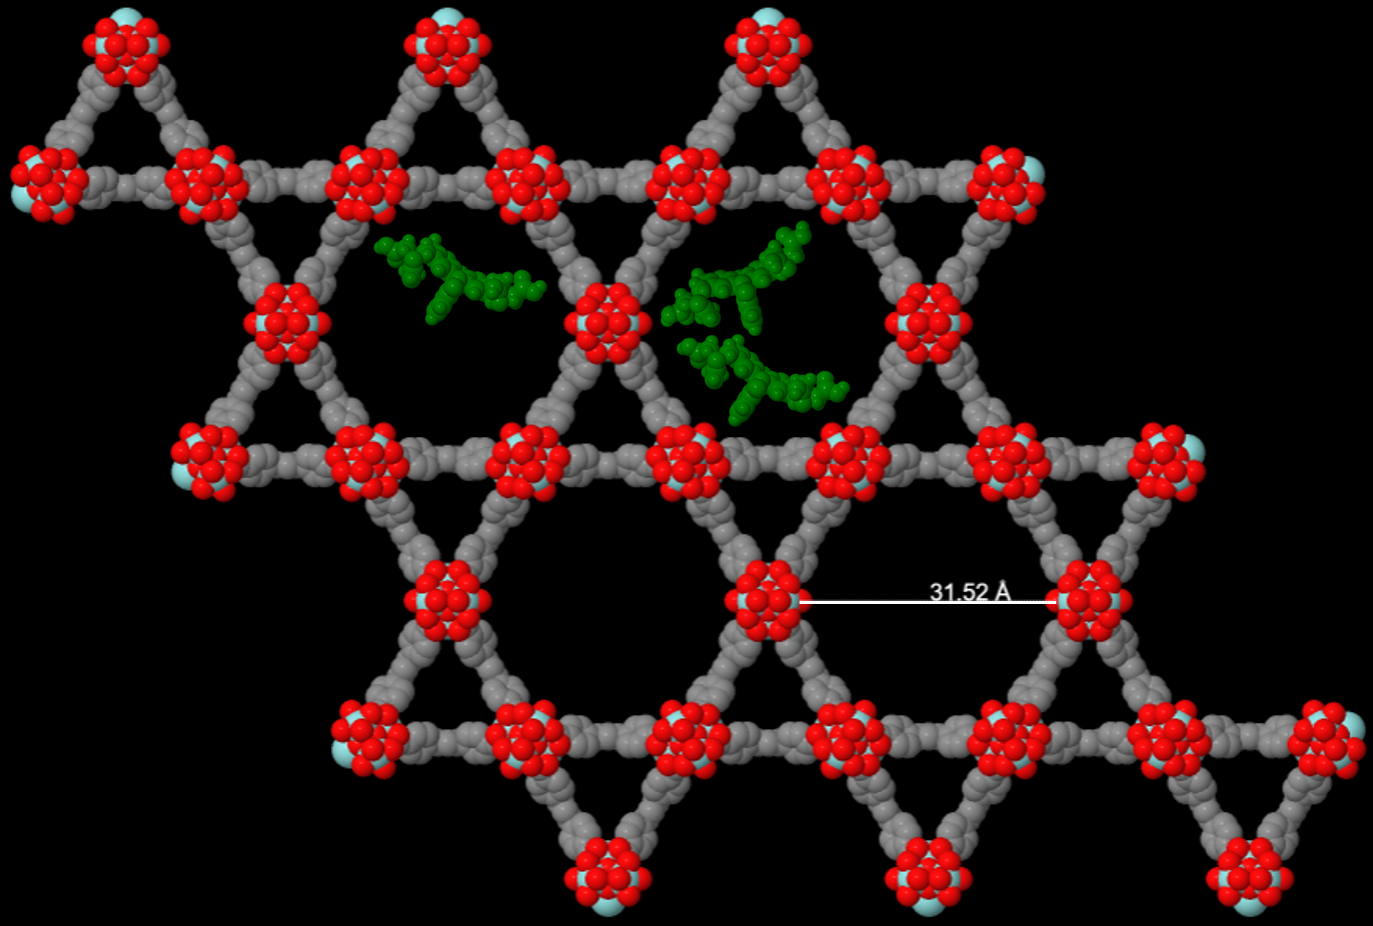
\includegraphics[width=1.0\textwidth]{calcein-in-MOF}
\caption[MOFs: The NU-1000 MOF has a large pore size to store other molecules]{MOFs are crystalline structures of metal ions joined by organic linkers. The pore size of NU-1000 MOF, \SI{31.5}{\angstrom}, is large enough to store calcein molecules shown here in green.}
\label{fig:calcein-in-MOF}
\end{figure}

If a MOF is used as the delivery system, the payload drug is stored in the pores of the MOF, as shown in Figure~\ref{fig:calcein-in-MOF}. 
It was hypothesised that, after loading the MOF with drug, release could be delayed by collapsing the pore structure. 
Pore collapse was achieved with a temperature treatment step after drug loading, before to the cells and imaging. 

In this experiement a naturally fluorescent dye, calcein, was used as a model drug. 
MOFs developed by Norwestern University, known as NU-1000 and NU-901, were chosen and synthesised for their large pore size. 
Calcein was loaded into the MOFs by soaking \SI{10}{\milli\gram} of either NU-1000 or NU-901 in a \SI[per-mode=symbol]{10}{\milli\gram\per\milli\litre} calcein solution for 3\,days in a \SI{37}{\degreeCelsius} shaking incubator. 
After this period, the supernatant was removed through centrifuging, and dried at \SI{37}{\degreeCelsius} for \SI{24}{\hour}. 

Temperature treatment was then performed on non-control samples. 
Samples were placed in a high-temperature vacuum oven at \SI{180}{\degreeCelsius} for \SI{24}{\hour} to induce pore collapse. 

\begin{figure}[htbp!]
\centering
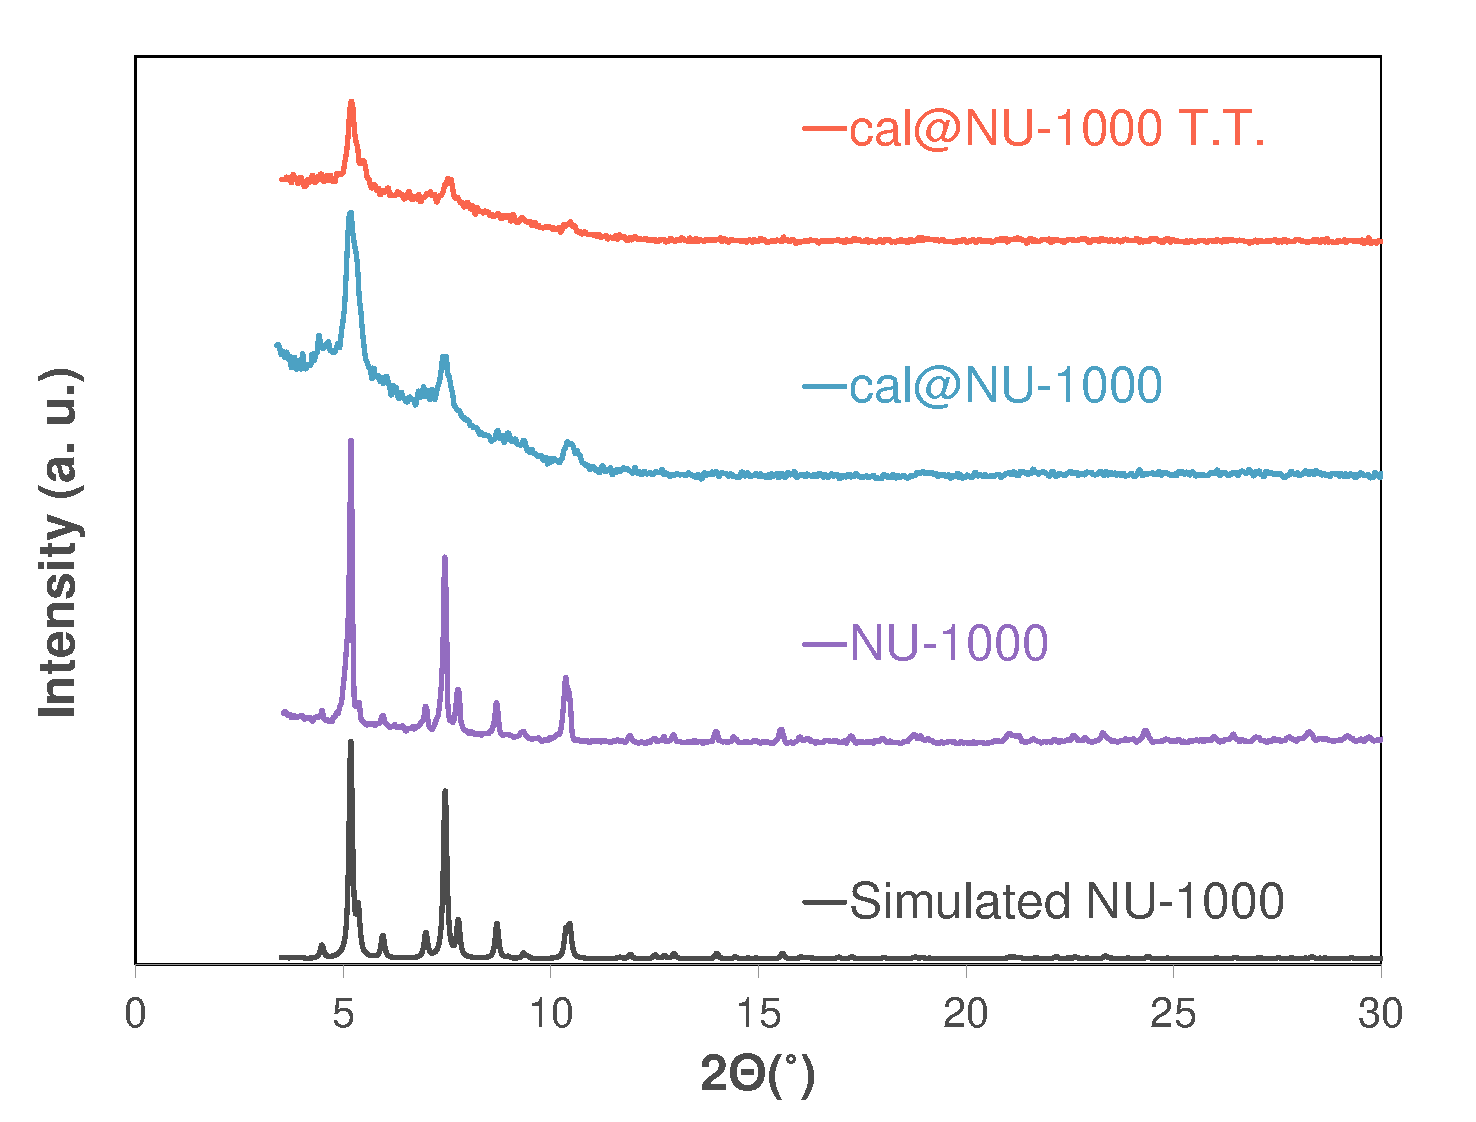
\includegraphics[width=0.7\textwidth]{pxrf-calcein-nu1000}
\caption[MOFs: PXRF confirms calcein enters NU-1000 and temperature treatment causes partial pore collapse]{ Experimental PXRF data (purple) matches well to simulated data (black). When calcein is loaded as a model drug (blue) the same Bragg peaks are still visible, showing that the crystalline structure is maintained; however the slight broadening of the peaks suggests calcein is successfully loaded into the MOF pores. After temperature treatment (red), pore collapse reduces the intensity of the peaks; however they are still visible, suggesting long-range crystalline order is preserved. }
\label{fig:MOF-PXRF}
\end{figure}

Pore collapse was verified by power X-ray diffraction patterns. 
Figure~\ref{fig:MOF-PXRF} shows that Bragg peaks broaden on addition of calcein, but are still visible at the same $\theta$, confirming the overall MOF structure is maintained. 
The slight broadening of loaded MOF is most likely a result of the loading process, which leads to some decrystallisation of the MOF. 
The decrease in peak intensity for temperature-treated MOF is due to a loss of crystalline structure from the pore collapse; however peaks are still visible, suggesting that long-range order was not completely destroyed.
This is in contrast to previous work, which induced pore collapse by mechanical amorphisation, causing peaks to completely disappear~\cite{orellana2015amorphous}.

The release profile of calcein from NU-1000 MOF is shown in Figure~\ref{fig:calcein-release-profile}, with the inset graph highlighting the burst release effect and its delay by temperature treatment. 
The effect of temperature treatment is particularly notable at the \SI{24}{\hour} time point, where MOF has only released 30\% of its payload, compared with 60\% released by untreated MOF.
This shows that the temperature treatment is successfully suppressing the burst release effect. 
% A bit of explanation about how this figure was made. FACS? - actually, general flow cytometry. Although this is a pretty generic term
 
\begin{figure}[htbp!]
\centering
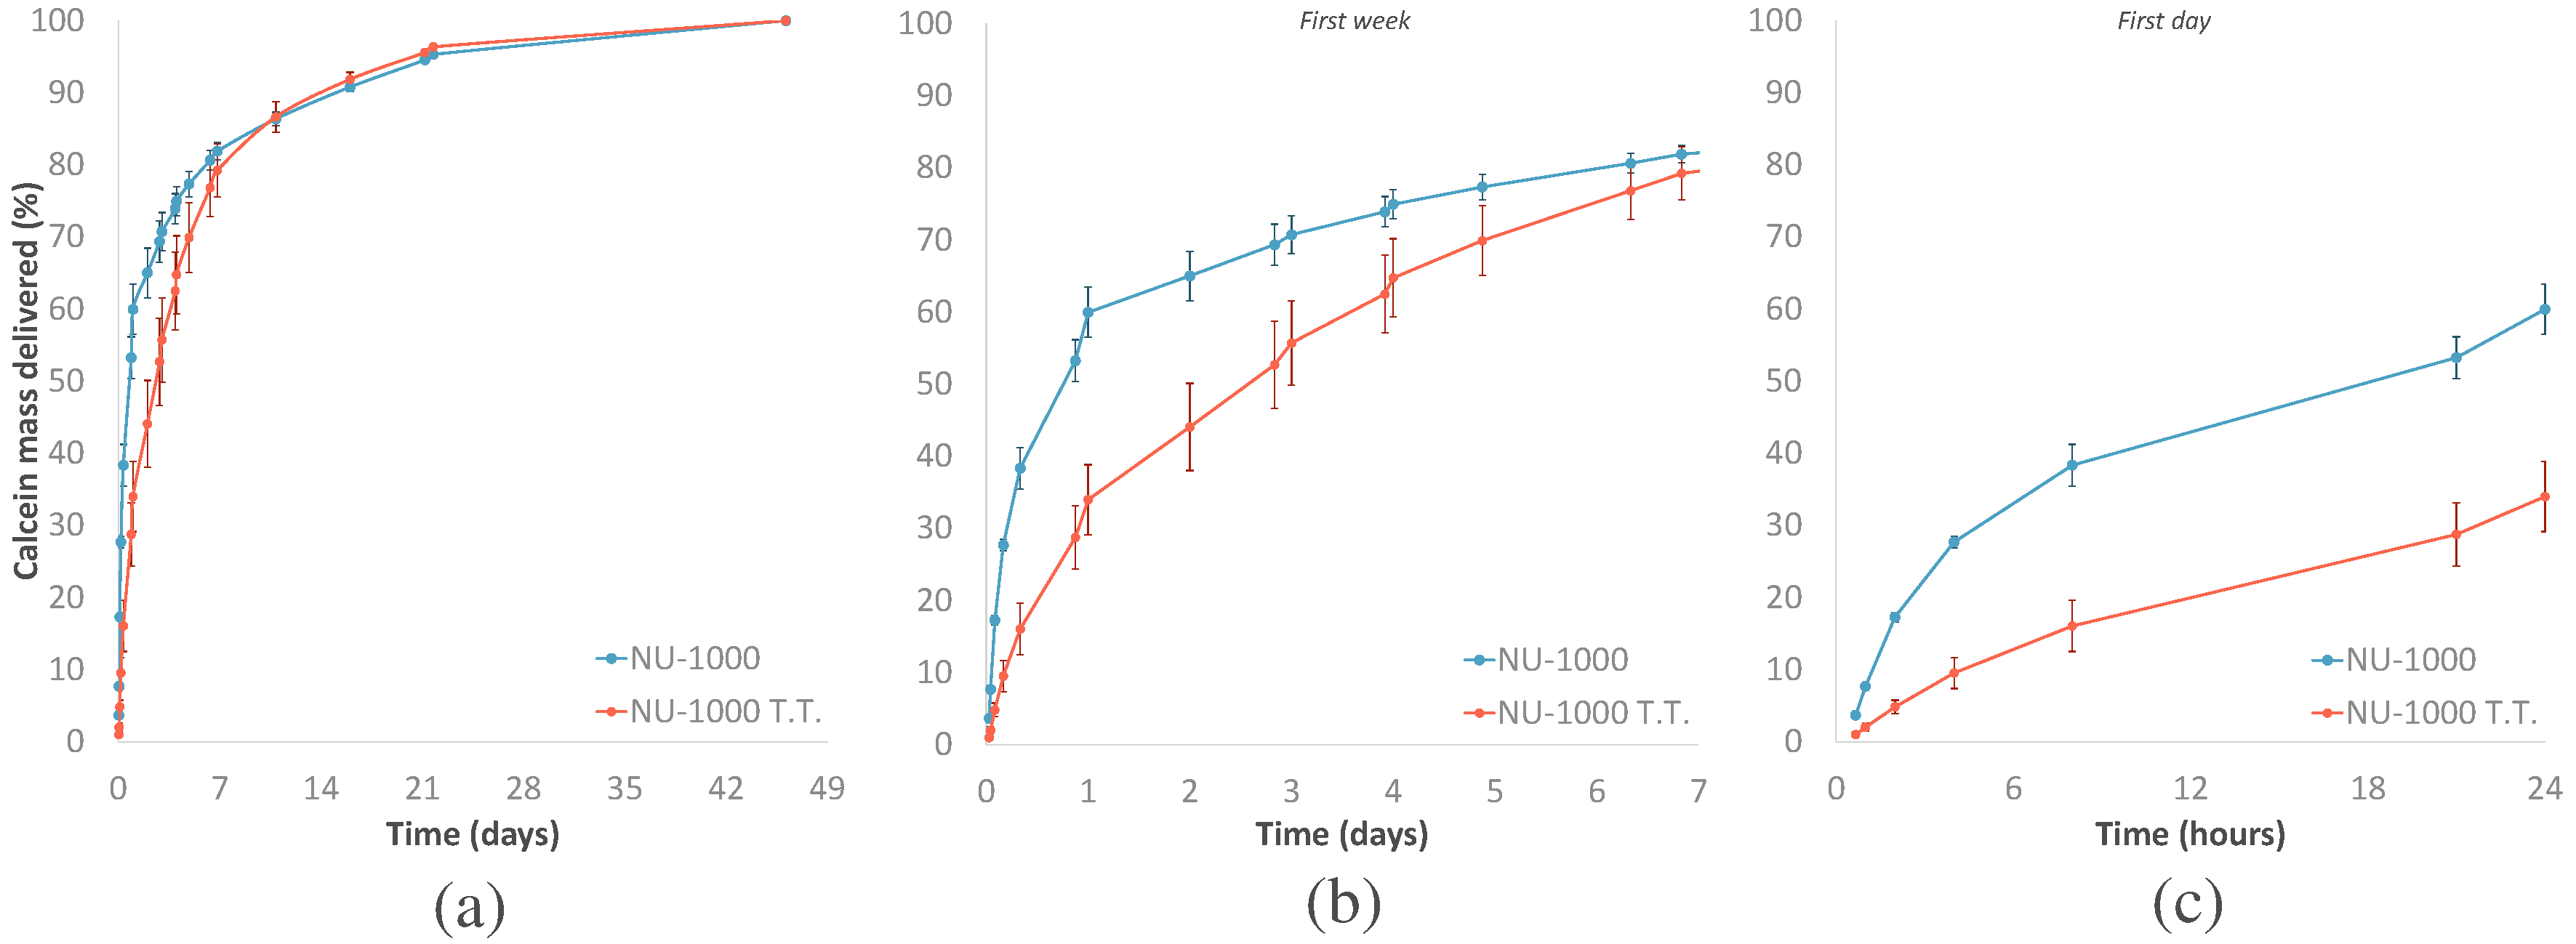
\includegraphics[width=1.0\textwidth]{calcein-release-profile}
\caption[MOFs: Payload release is delayed by temperature treatment]{ The figure shows three views of the same graph, with the time axis scaled differently to highlight the delay of payload release from MOF. The effect is particularly noticeable after \SI{24}{\hour}, where just 30\% of the payload is released from temperature-treated MOF compared to 60\% released from untreated MOF. By delaying the release the MOF has longer to enter cells and will deliver a higher percentage of its payload, rather than releasing it in extracellular space. }
\label{fig:calcein-release-profile}
\end{figure}

In order to visualise calcein release in a biological context, HeLa cells were labelled with HCS NuclearMask™ Deep Red Stain to view the nucleus, and CellLight Lysosomes-RFP BacMam 2.0 or CellLight Early Endosomes-RFP BacMam 2.0 to view lysosomes or endosomes respectively. 
Calcein itself is fluorescent at 495/515\,\si{\nano\meter} for excitation and emission wavelengths respectively, so had good spectral separation for imaging in 3-colours. % Need to cite this somehow, thermofisher?

Images were captured on the LAG SIM, utilising optical sectioning to remove out of focus light. 
Representative image slices over a \SI{24}{\hour} period are shown in Figure~\ref{fig:calcein-MOF-uptake}. 
Note that the nucleus was not captured for most images to minimise imaging time and thus prolong cell viability; a 3-colour image is presented in the SIM showcase, Figure~\ref{fig:recon-mofcell}. 
Also notable is that the MOF is highly autofluorescent at the same wavelength as calcein, such that the calcein released from the MOF cannot be seen on its own. 
In later experiments, detailed in Section~\ref{sec:MOF-siRNA}, a drug with better spectral separation was used for clearer imaging.

\begin{figure}[tbp]
\centering
\begin{subfigure}[b]{0.325\textwidth}
	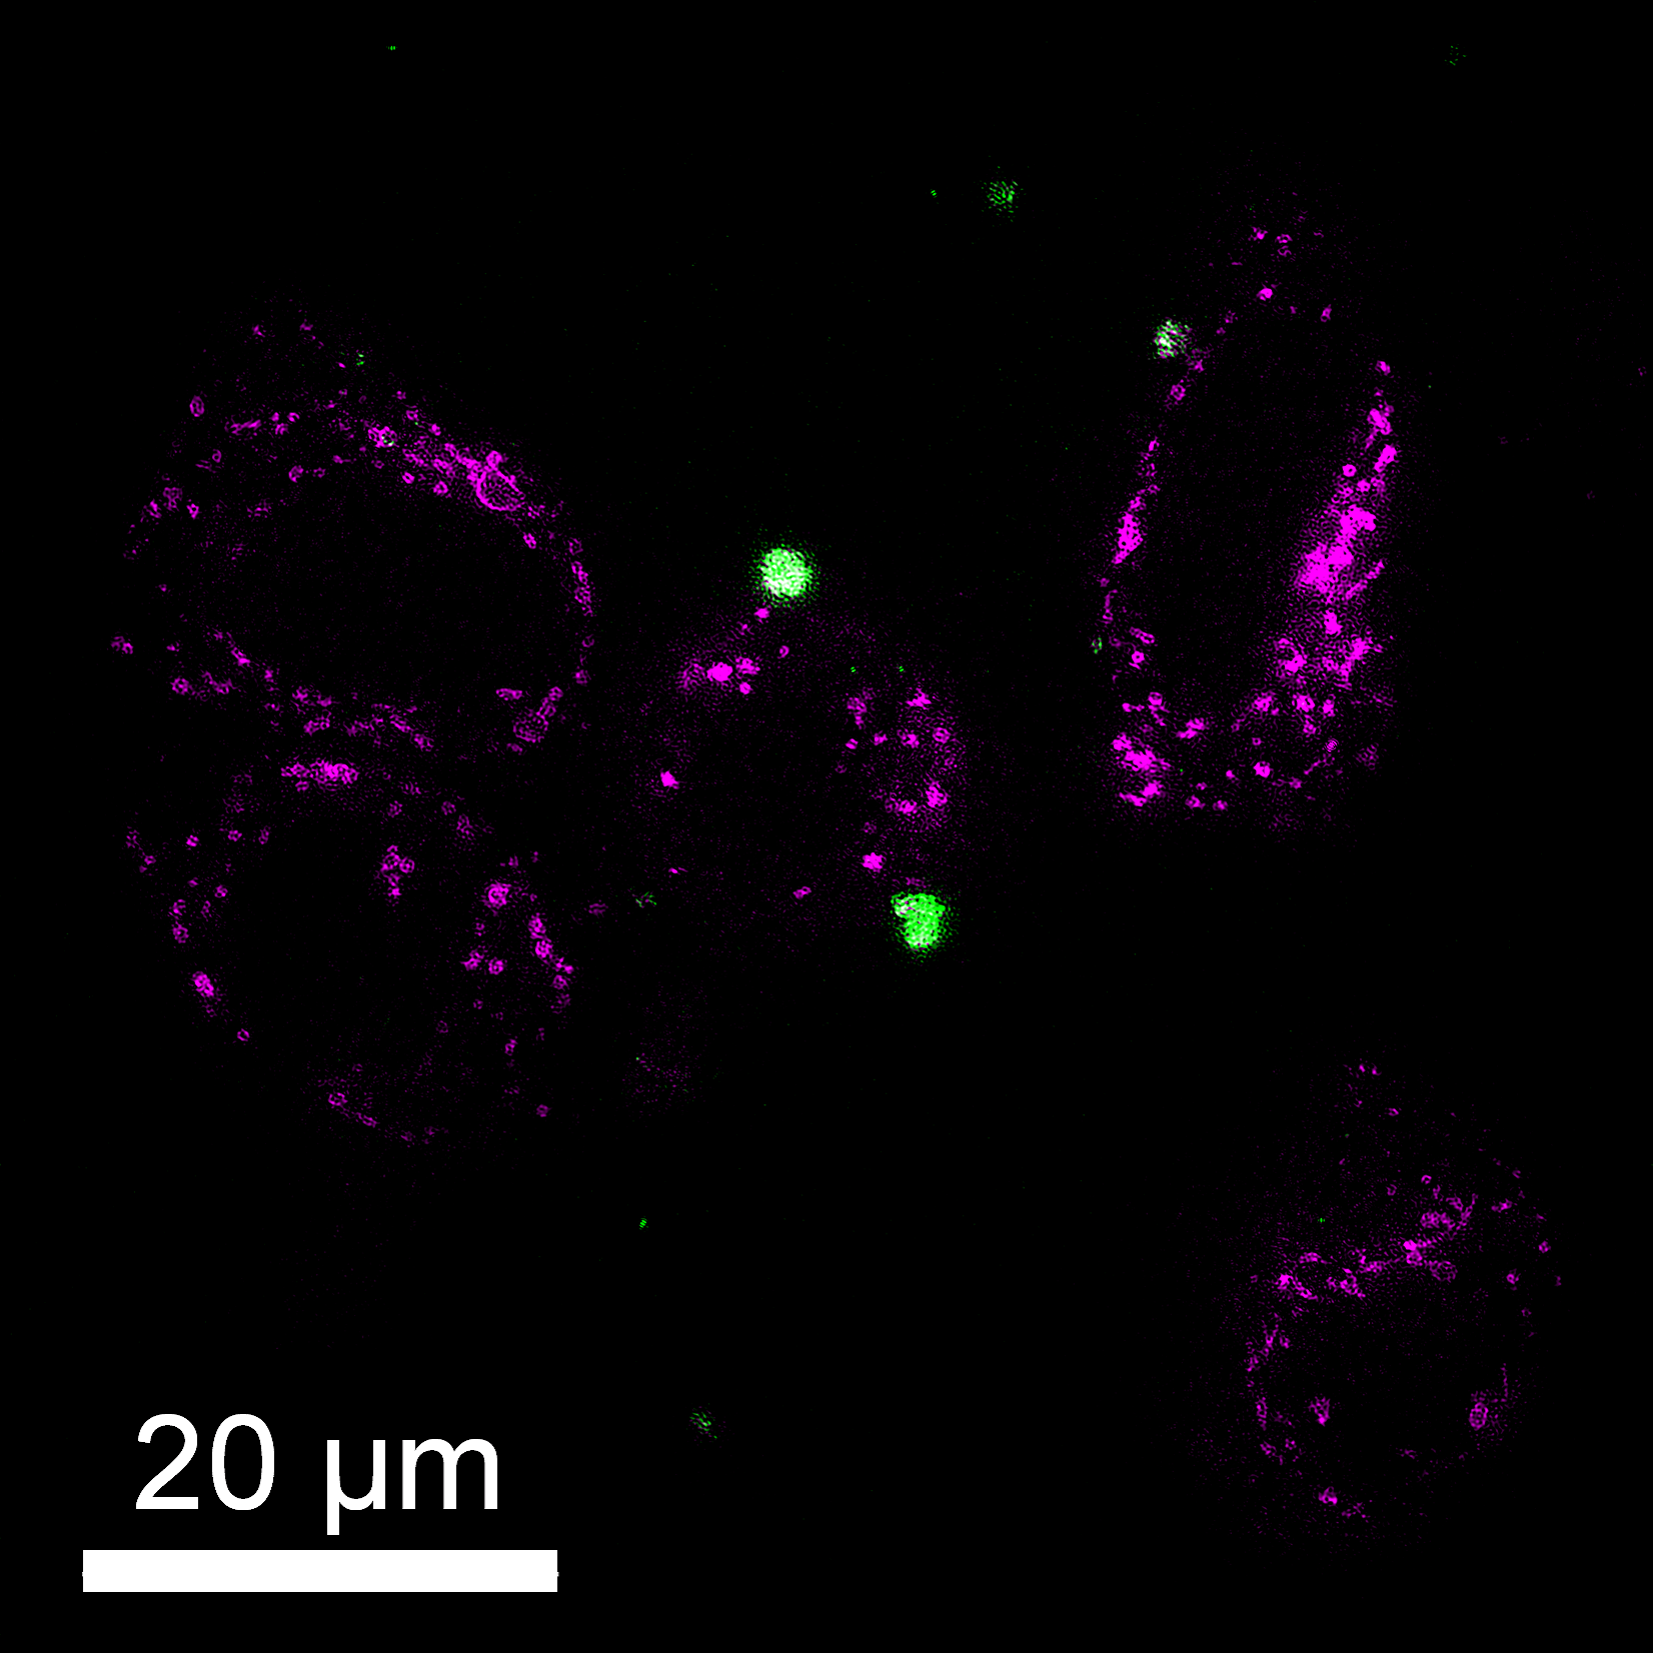
\includegraphics[width=\textwidth]{calcein-MOF-uptake-1}
	\caption{30\,minutes}\label{fig:calcein-MOF-uptake-1}
\end{subfigure}
\hfill
\begin{subfigure}[b]{0.325\textwidth}
	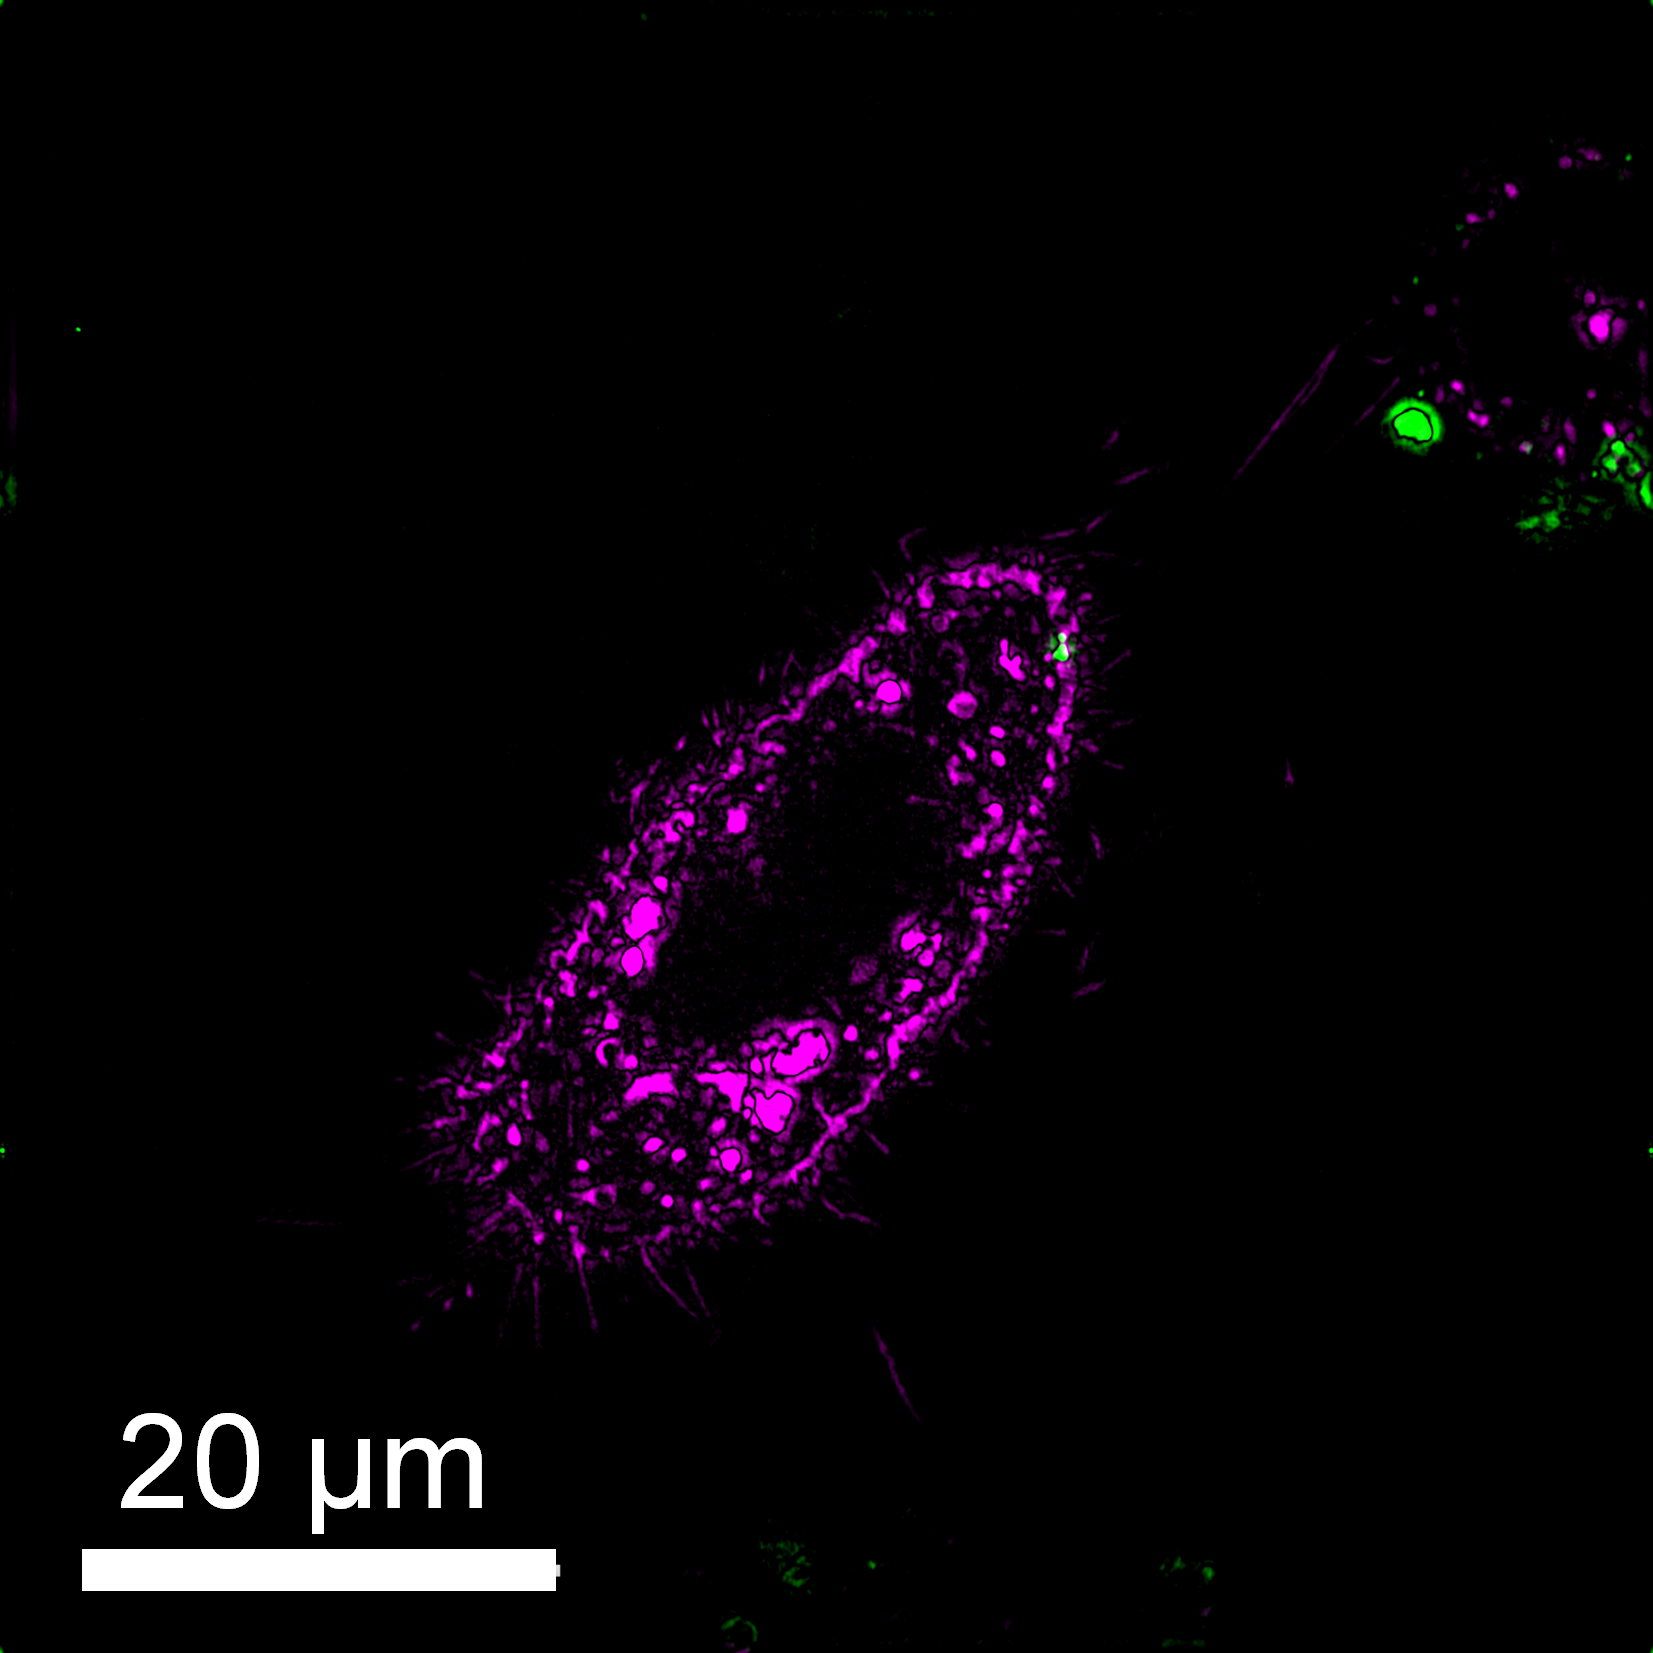
\includegraphics[width=\textwidth]{calcein-MOF-uptake-2}
	\caption{1\,hour}\label{fig:calcein-MOF-uptake-2}
\end{subfigure}
\hfill
\begin{subfigure}[b]{0.325\textwidth}
	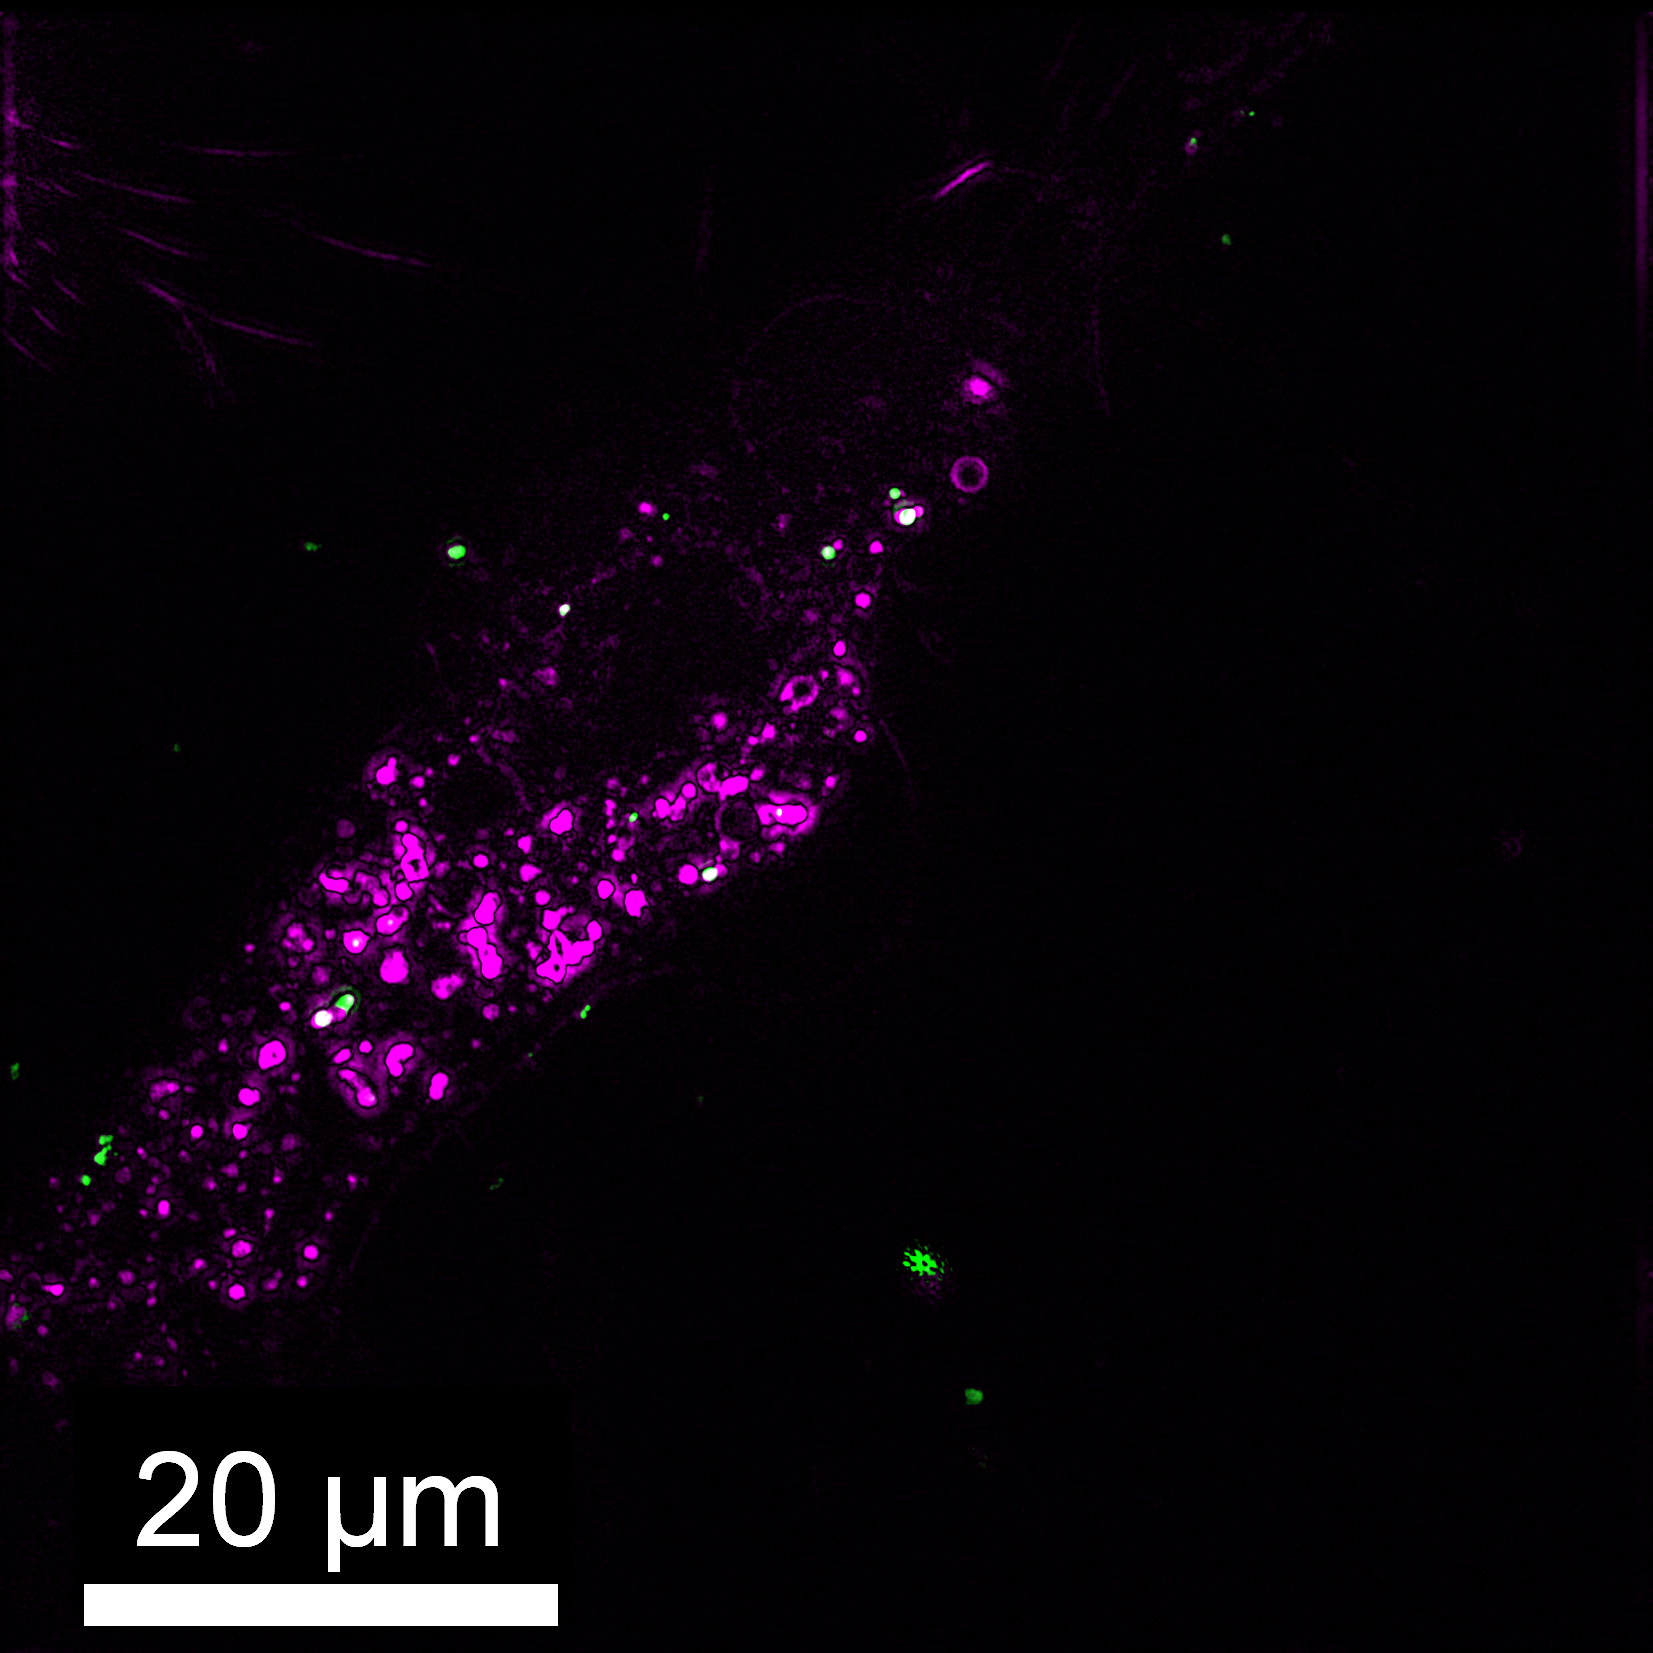
\includegraphics[width=\textwidth]{calcein-MOF-uptake-3}
	\caption{2\,hours}\label{fig:calcein-MOF-uptake-3}
\end{subfigure}

~\newline
\begin{subfigure}[b]{0.325\textwidth}
	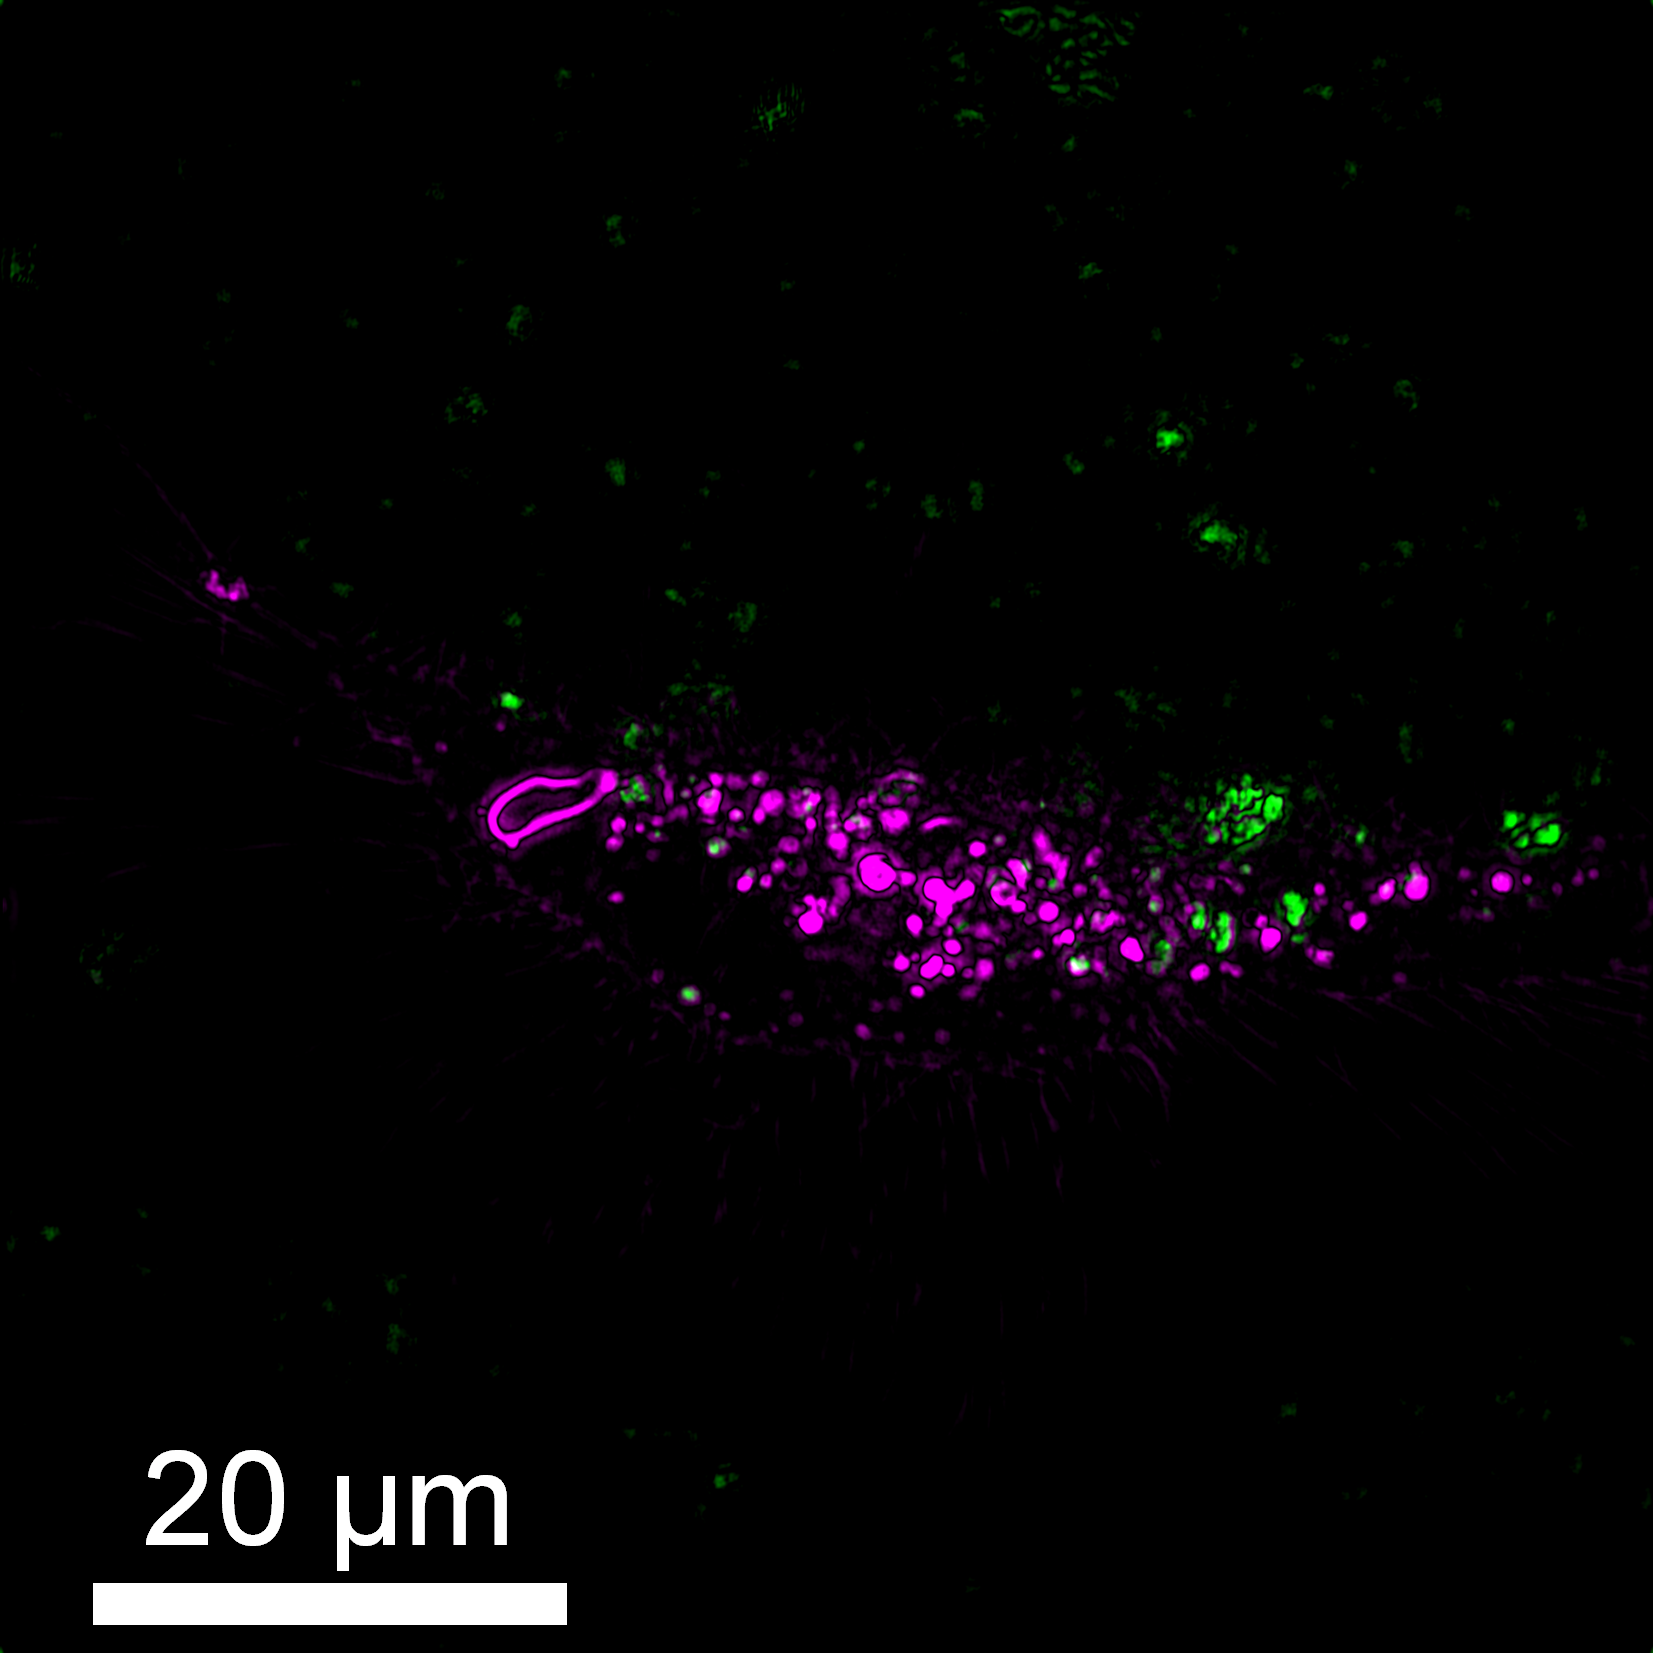
\includegraphics[width=\textwidth]{calcein-MOF-uptake-4}
	\caption{6\,hours}\label{fig:calcein-MOF-uptake-4}
\end{subfigure}
\hfill
\begin{subfigure}[b]{0.325\textwidth}
	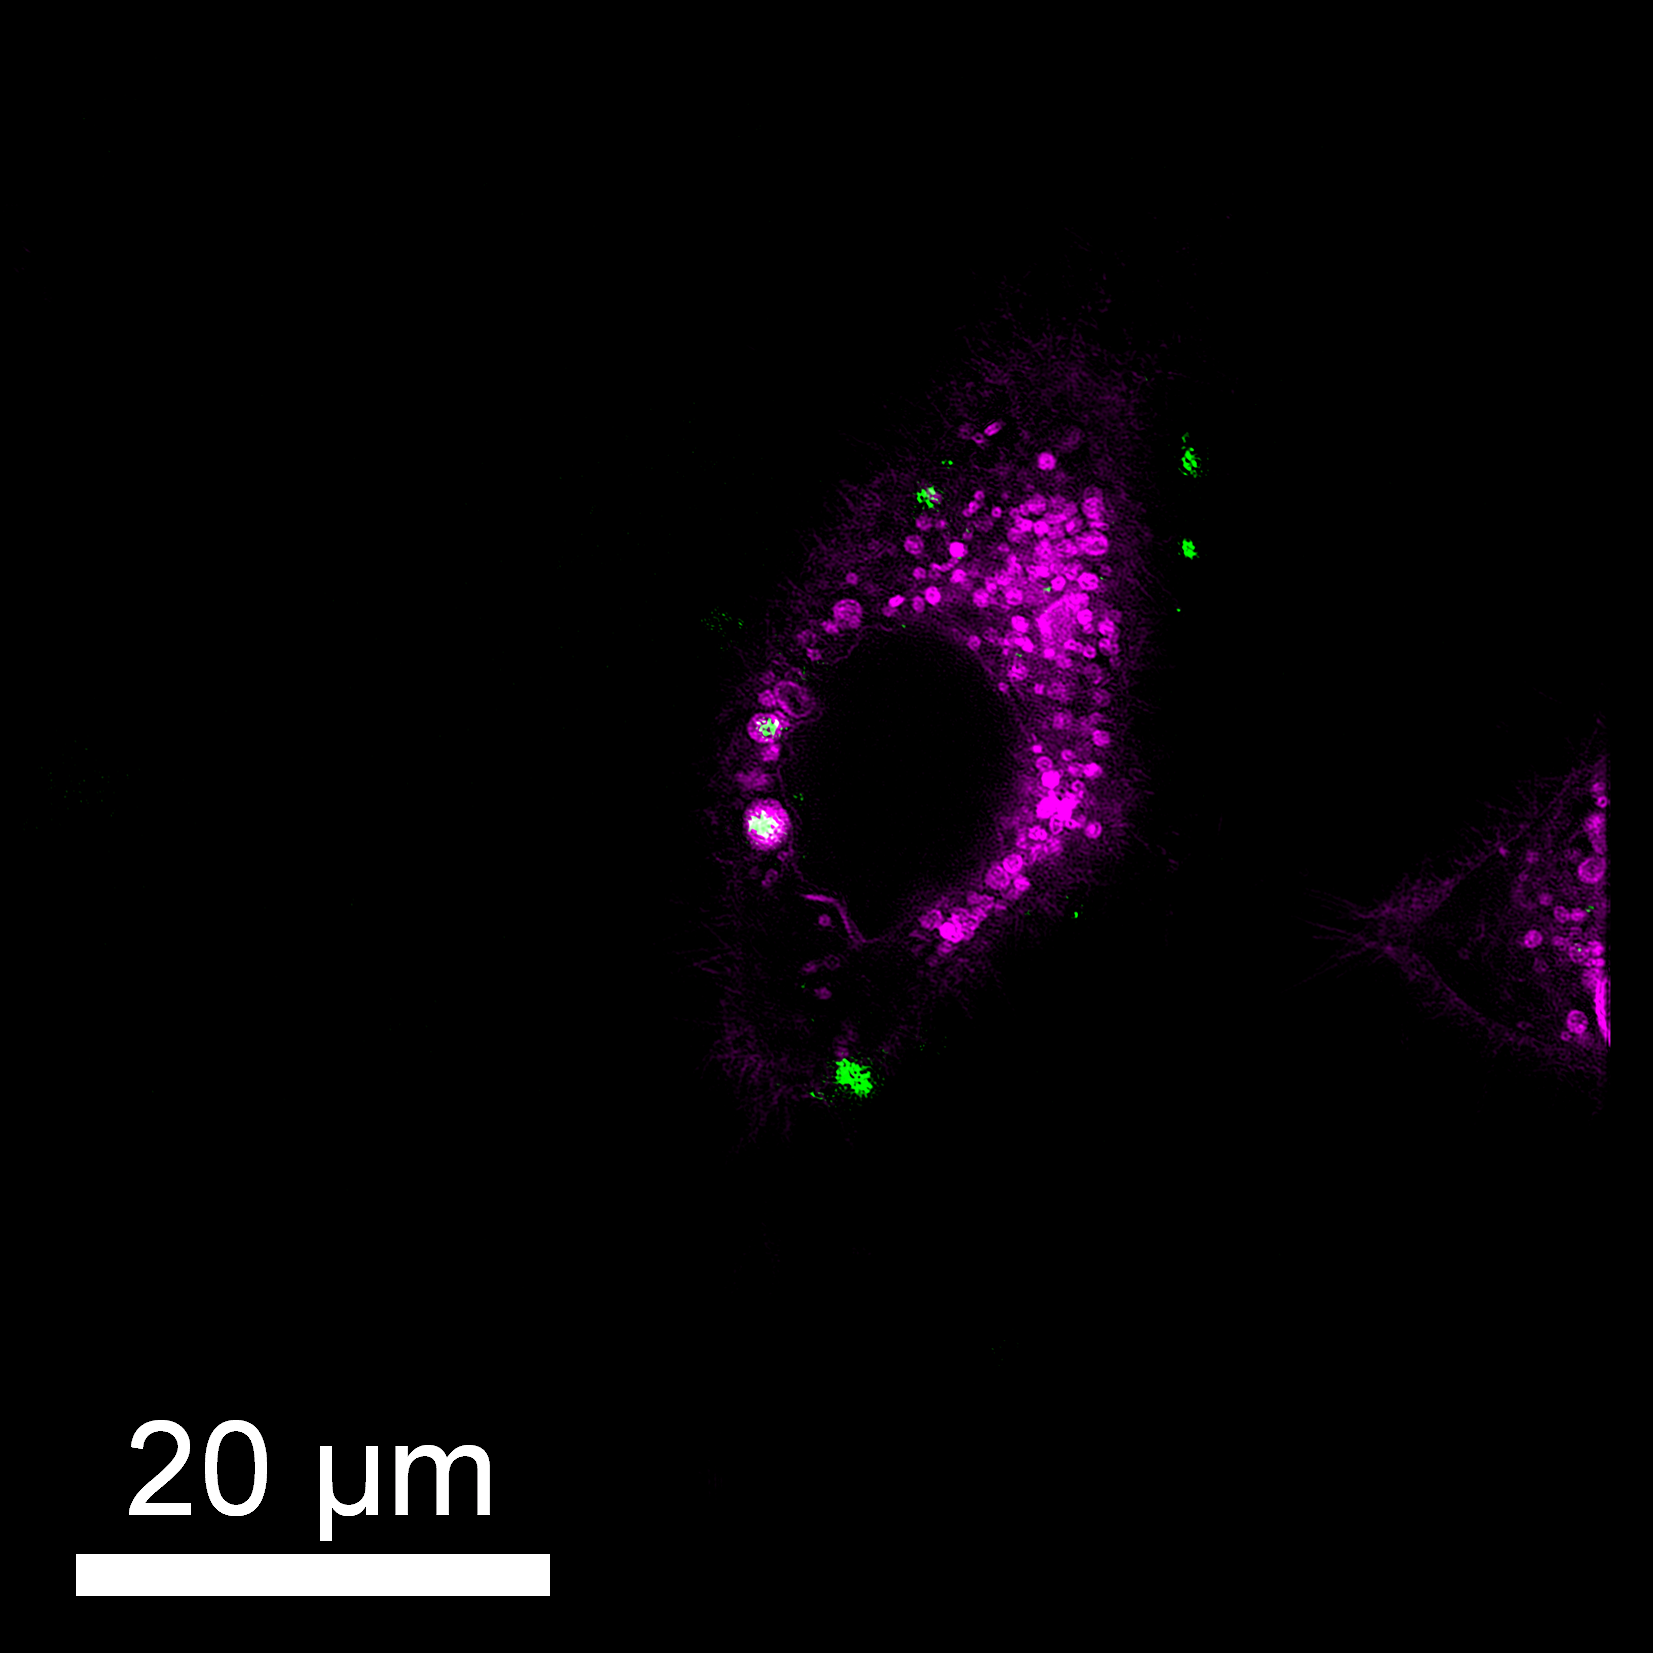
\includegraphics[width=\textwidth]{calcein-MOF-uptake-5}
	\caption{8\,hours}\label{fig:calcein-MOF-uptake-5}
\end{subfigure}
\hfill
\begin{subfigure}[b]{0.325\textwidth}
	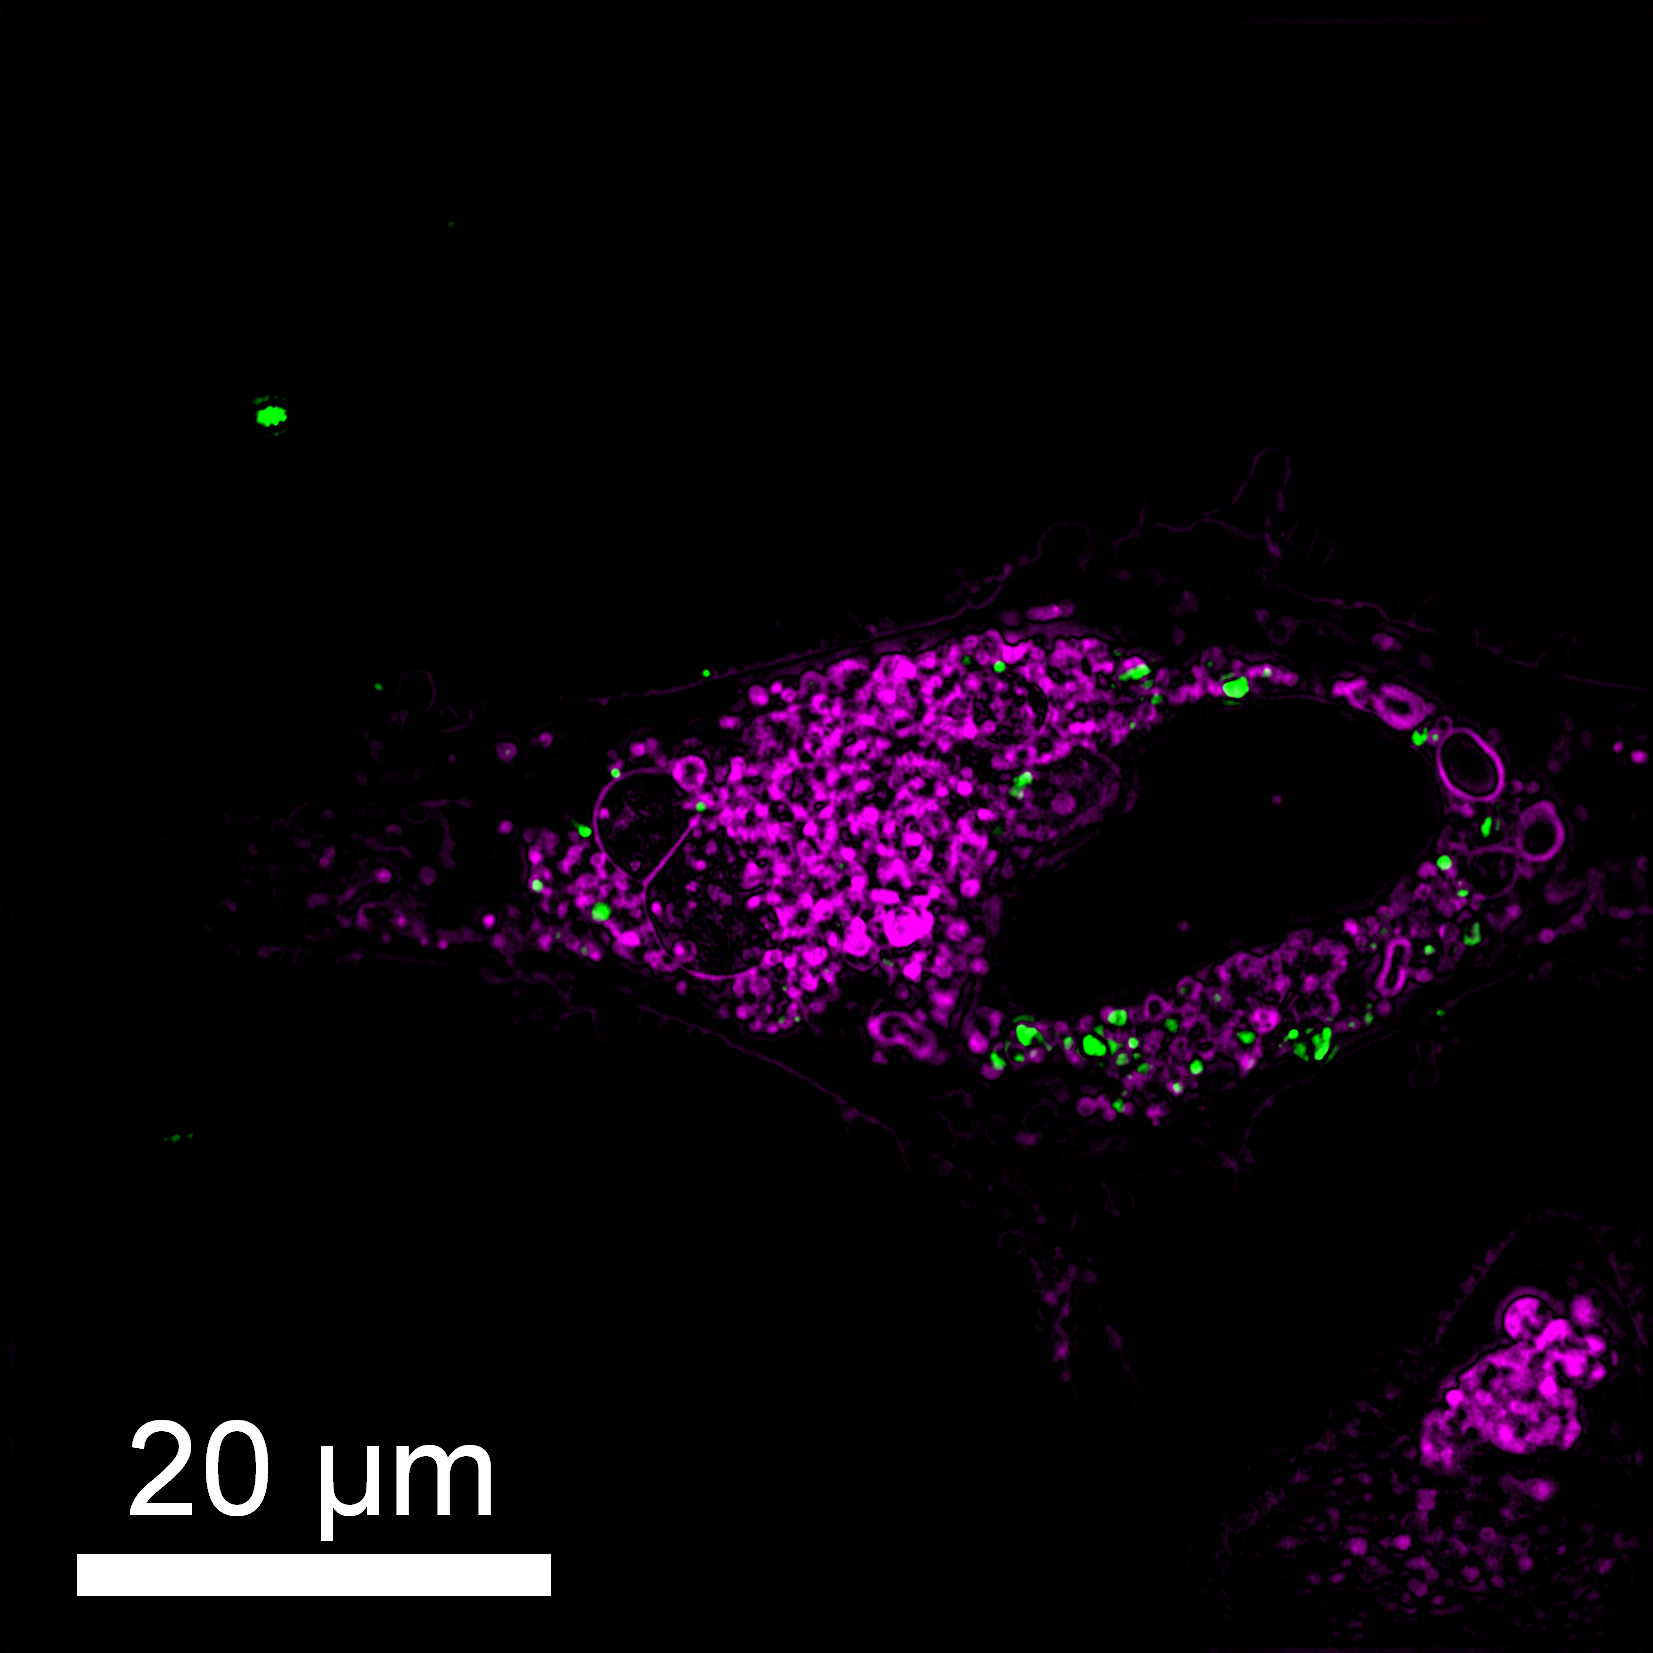
\includegraphics[width=\textwidth]{calcein-MOF-uptake-6}
	\caption{24\,hours}\label{fig:calcein-MOF-uptake-6}
\end{subfigure}
\caption[MOFs: Calcein-loaded NU-1000 is taken up by cells over a \SI{24}{\hour} period]{Images of Hela cells, with endosomes coloured in magenta, captured over a ~\SI{24}{\hour} time period show the successful uptake of calcein-loaded NU-1000, coloured in green. The low quantity of uptake in the first \SI{2}{\hour} highlights the need for temperature treatment to delay payload release, avoiding the burst release effect. These images can be viewed interactively in 3D at \url{https://fpb.ceb.cam.ac.uk/MOF} to confirm MOF is located within the cells, and not simply sitting on the cell membrane. }
\label{fig:calcein-MOF-uptake}
\end{figure}

An issue with examining 2D image slices is that it is unclear whether MOF has entered the cell, or is simply sitting on the cell membrane with out-of-focus light making it appear localised within the cell. 
Optical sectioning allowed images to be reconstructed in 3D, so that the cell could be viewed from any angle, verifying that MOF had indeed been taken inside the cell. 
To allow readers of the publication to verify this themselves, full 3D reconstructions of the slices in Figure~\ref{fig:calcein-MOF-uptake} are hosted online with FPBioimage, and can be viewed at \url{https://fpb.ceb.cam.ac.uk/MOF/}. 

The slices in Figure~\ref{fig:calcein-MOF-uptake}, together with their online 3D visualisations, show that MOF is successfully taken up by HeLa cells over a \SI{24}{\hour} period. 
The MOF appears to be taken up by endocytosis, evident from the colocalisation of endosomes with MOFs, seen as white areas in the Figure. 
To verify this observation, an endocytosis study was performed.
Inhibitors of various endocytosis pathways were added to the cells, and the fluorescence in the cytoplasm measured after a \SI{24}{\hour} incubation period. 
Figure~\ref{fig:MOF-endocytosis-study} firstly confirms that MOF uptake is an active process, as reducing the temperature to \SI{4}{\degreeCelsius} causes a significant reduction in cytoplasmic fluorescence. 
Furthermore, the study shows that \SI{0.3}{\Molar} sucrose also causes a significant reduction in the amount of MOF uptake, implying MOF is endocytosed by the clathrin-mediated pathway. 

\begin{figure}[htbp!]
\centering
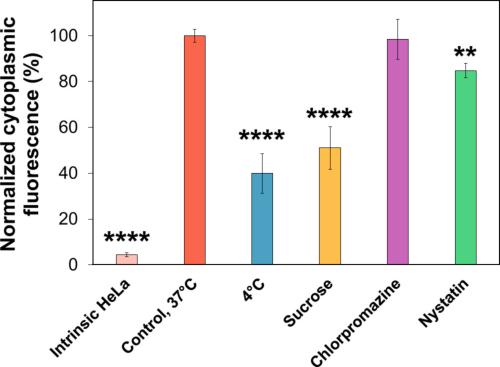
\includegraphics[width=1.0\textwidth]{endocytosis-study}
\caption[MOFs: An endocytosis study shows NU-1000 MOF is taken up by HeLa cells through the clathrin-mediated pathway]{Cytoplasmic fluorescence was measured after incubating cells with NU-1000 MOF for \SI{24}{\hour} under various conditions to measure how much MOF enters cells. The low bar after incubation at \SI{4}{\degreeCelsius} shows that MOF uptake is an active endocytosis process. The low bar after incubation with sucrose suggests MOF is endocytosed by the clathrin-mediated pathway. $****: p<0.0001$, $**: p<0.01$. }
\label{fig:endocytosis-study}
\end{figure}

Further evidence of endocytosis is provided by video-rate imaging of MOF uptake.
Supplementary video 3 shows that MOF outside the cell moves with fast Brownian motion; once inside the cell, however, MOF is comparitvely static. 
This provides further evidence that MOF is taken up by the cells to deliver its payload. 

The timescale over which MOF enters cells is important, and emphasises the need for the temperature treatment process. 
Figure~\ref{fig:calcein-release-profile} shows that, without temperature treatment, 30\% of the payload is released within the first \SI{4}{\hour}. 
The timelapse images in Figure~\ref{fig:calcein-MOF-uptake} show that very little MOF has entered the cell by this time, indicating that the calcein payload has been dumped in extracellular space. 
For a real drug, this would significantly reduce theraputic effect. % waste of concentration, potentially reach toxic levels of concentration too early. Temperature treatment will allow lower concentrations. Result. Yay! 


\subsection{Loading MOFs with siRNA for therapeutic effects} \label{sec:MOF-siRNA}
To quantify the therapeutic effect of delivering drugs to cells using MOFs, we loaded NU-1000 MOFs with small interfering ribonucleic acids (siRNA). 

A HEK-293 cell line with the T-REx Flp-In™ system was used to express the fluorescent protein mCherry. 
Under normal conditions therefore, these cells are fluorescent at 587/610\,\si{\nano\meter} for excitation and emission wavelengths respectively. 

An siRNA sequence was designed to cleave the mRNA molecule and suppress expression of the mCherry protein.
The 21-nucleotide-long sense strand which was most effective at suppressing fluorescent emission was 5'-AAGGAGTTCATGCGCTTCAAG-3'. 
Scrambled siRNA, used as a negative control, did not cause any suppression of fluorescence.
A combination of mCherry-fluorescent HEK-293 cells and mCherry-targeting siRNA creates a model drug delivery system which is quantifiable: the lower the fluorescence, the more effective the siRNA is at suppressing gene expression. 

Without MOF, Figure~\ref{fig:mof-enzyme-degradation} shows that siRNA is broken down by enzymes present in extra-celluar space - in this case, RNase~\cite{chirgwin1979isolation}.
When the siRNA is loaded into MOF, it is protected from enzymes, demonstrated by the retention of a mark mark at \SI{21}{nt}. 
The retention and broadening of low-$\theta$ peaks in Figure~\ref{fig:mof-enzyme-pxrd} confirms that the MOF is loaded inside the pores of the MOF, which protects it from enzymes. 

\begin{figure}[htbp!]
	\centering
	\begin{subfigure}[b]{0.49\textwidth}
		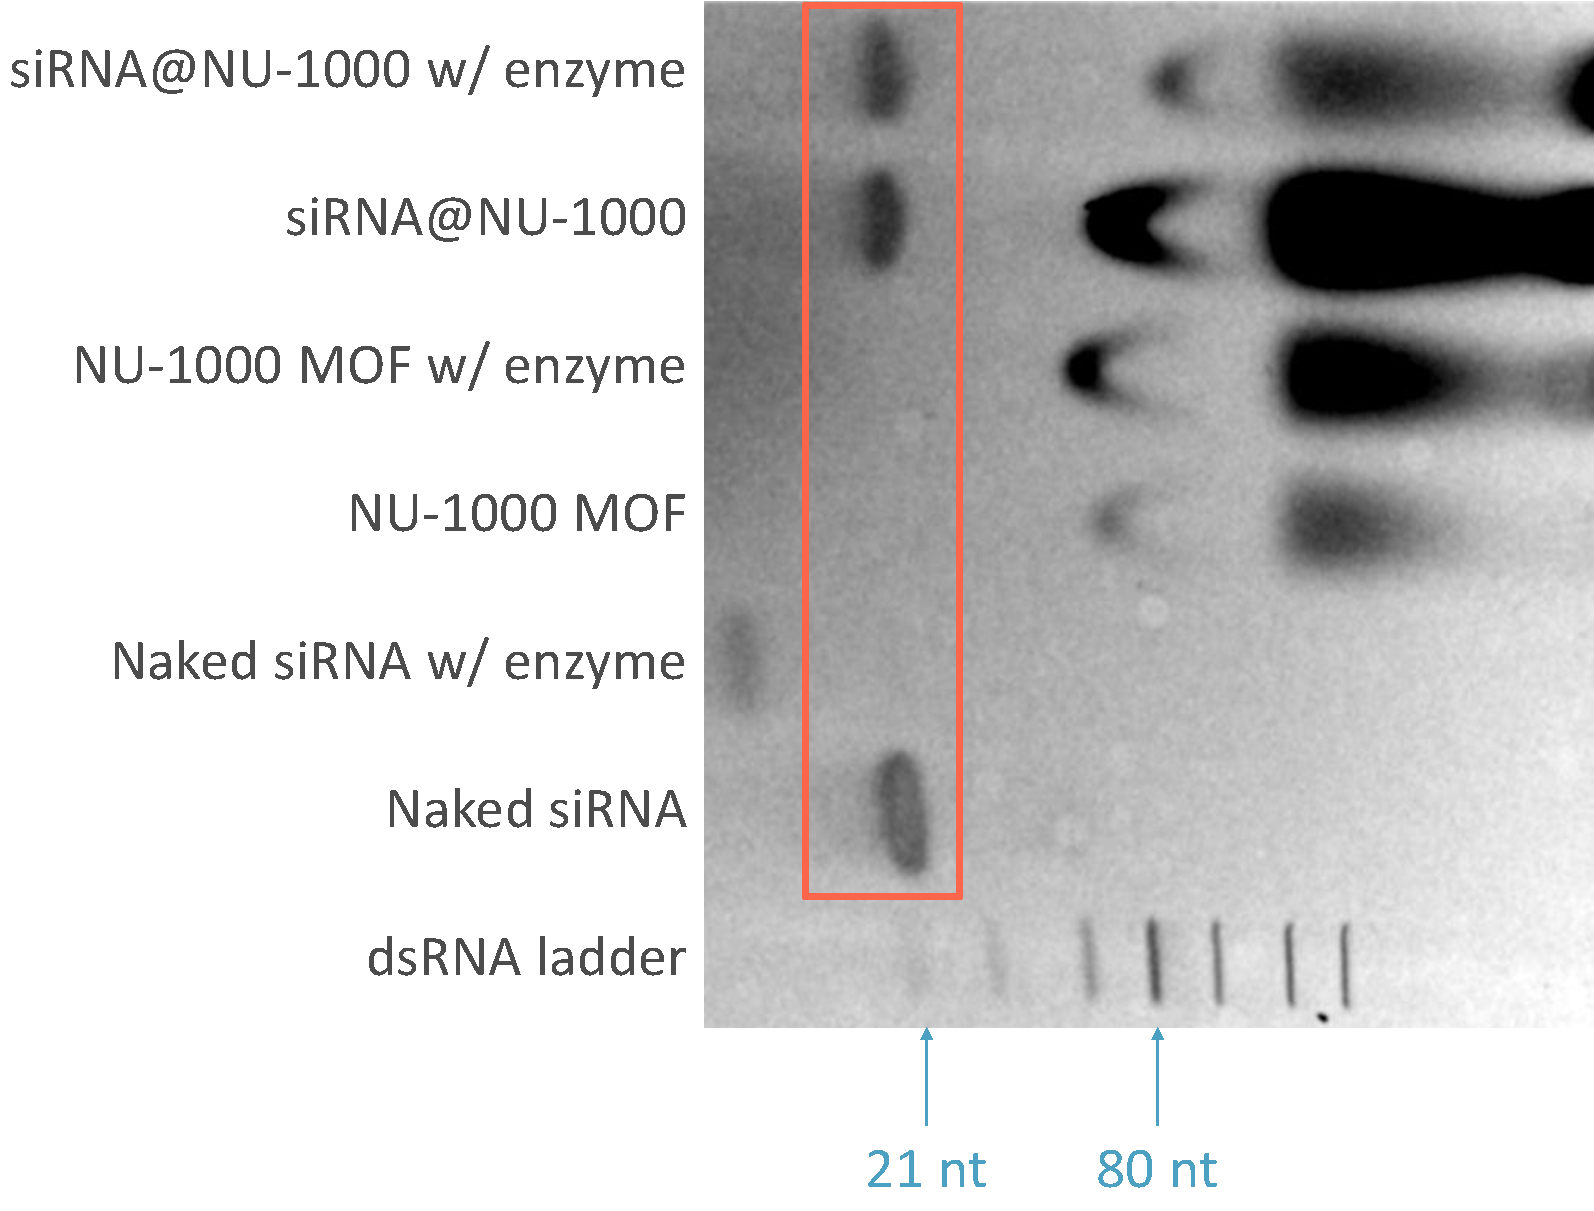
\includegraphics[width=1.0\textwidth]{mof-enzyme-degradation}
		\caption{} \label{fig:mof-enzyme-degradation}
	\end{subfigure}
	\hfill
	\begin{subfigure}[b]{0.49\textwidth}
		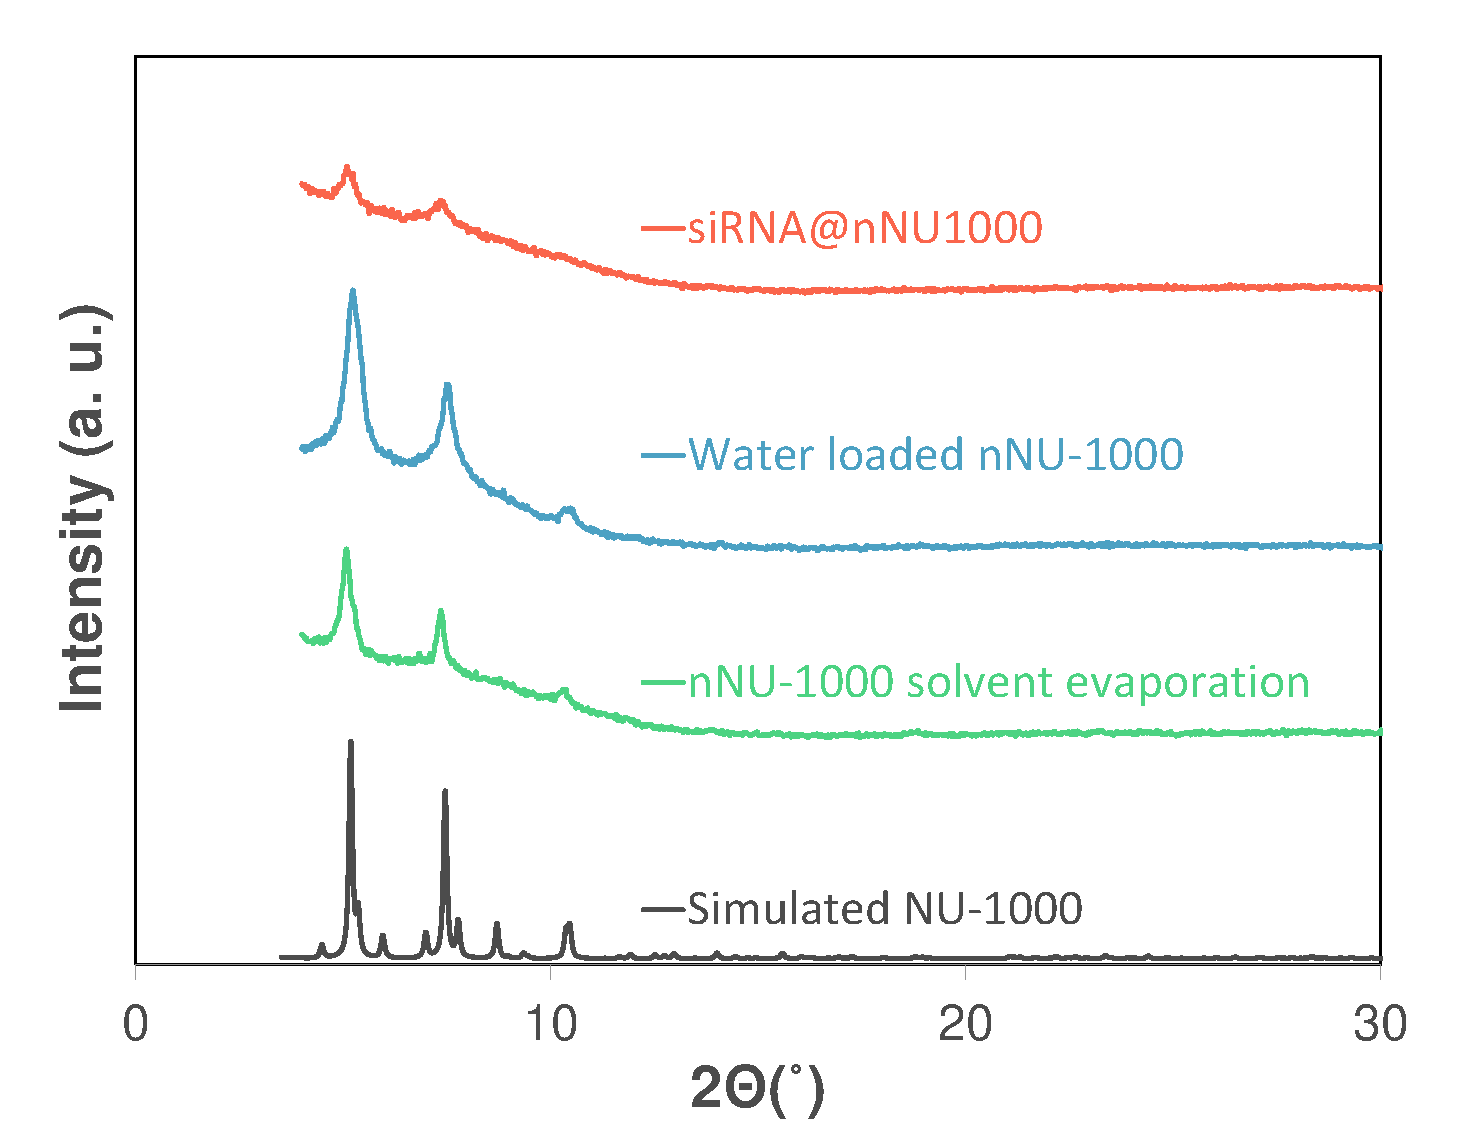
\includegraphics[width=1.0\textwidth]{mof-sirna-pxrd}
		\caption{} \label{fig:mof-sirna-pxrd}
	\end{subfigure}			
	\caption[MOFs: NU-1000 protects siRNA from degradation by enzymes in extracellular space]{The gel in (a) has a mark at \SI{21}{nt} when siRNA is present. When RNAase is added to the system, naked siRNA is broken down and not mark is present. Loading siRNA into NU-1000 protects the siRNA from degradation, and the mark at \SI{21}{nt} is retained. PXRD plots shown in (b) confirm siRNA is contained within the pores of NU-1000, shown by broadening of the Bragg peaks.}
\label{fig:mof-enzyme-pxrd}
\end{figure}

To confirm that siRNA-loaded MOF could enter cells, we used LAG SIM to image cells, MOF, and siRNA. 
As seen in Section~\ref{sec:mof-temperature}, this MOF is naturally fluorescent at \SI{488}{\nano\metre}. 
The CellLight Early Endosomes-RFP BacMam 2.0 stain was used to visualise endosomes in cells. 
An Alexa Fluor 647 was tagged onto the 5' end of the siRNA sense strand. 
Multi-colour SIM imaging could then be used to assess cellular uptake of the MOF complex, and confirm that siRNA could enter the cell. 

Figure~\ref{fig:siRNA-MOF-uptake} shows MOF uptake experiments under four conditions, after \SI{4}{\hour} of incubation. 
MOF is coloured in green, endosomes in blue, and siRNA in red. 


\begin{figure}[tbp]
\centering
\begin{subfigure}[b]{0.49\textwidth}
	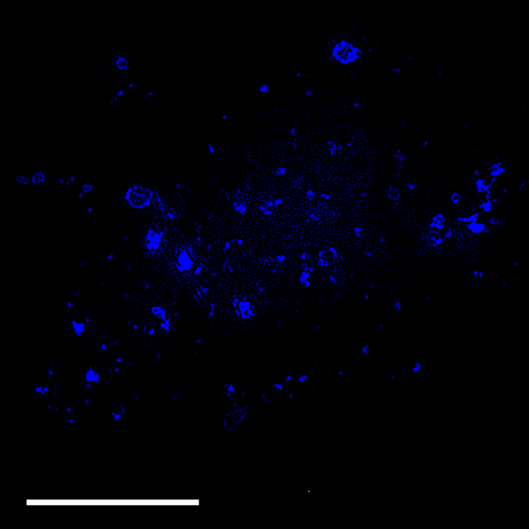
\includegraphics[width=\textwidth]{siRNA-MOF-uptake-1}
	\caption{}\label{fig:siRNA-MOF-uptake-1}
\end{subfigure}
\hfill
\begin{subfigure}[b]{0.49\textwidth}
	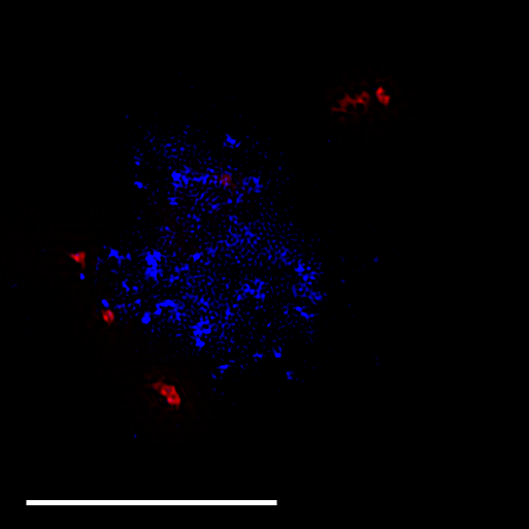
\includegraphics[width=\textwidth]{siRNA-MOF-uptake-2}
	\caption{}\label{fig:siRNA-MOF-uptake-2}
\end{subfigure}

~\newline
\begin{subfigure}[b]{0.49\textwidth}
	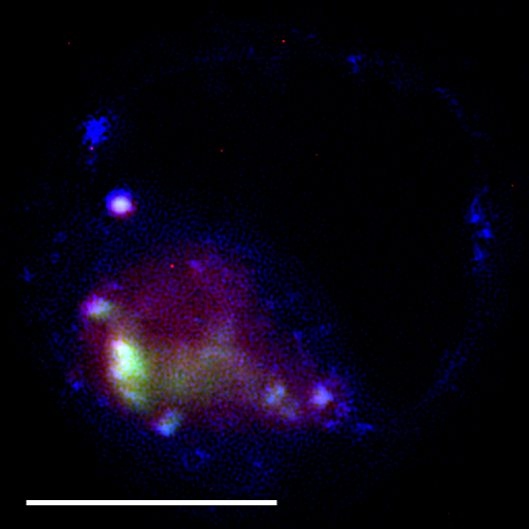
\includegraphics[width=\textwidth]{siRNA-MOF-uptake-3}
	\caption{}\label{fig:siRNA-MOF-uptake-3}
\end{subfigure}
\hfill
\begin{subfigure}[b]{0.49\textwidth}
	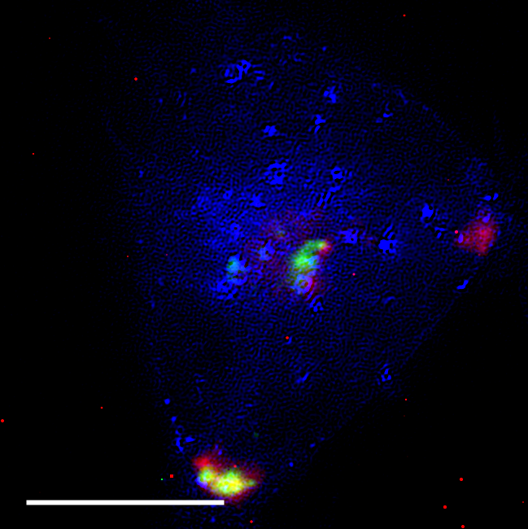
\includegraphics[width=\textwidth]{siRNA-MOF-uptake-4}
	\caption{}\label{fig:siRNA-MOF-uptake-4}
\end{subfigure}
\caption[MOFs: siRNA-loaded NU-1000 is endocytosed by HEK-293 cells, and released to the cytoplasm with an endosome release factor]{Images show endosomes coloured in blue, NU-1000 MOF in green, and siRNA in red, for HEK-293 cells incubated for \SI{4}{\hour} under different experimental conditions. (a) shows cells incubated with naked siRNA; the absence of red signal suggests siRNA is degraded in extra-cellular space. (b) shows siRNA loaded into Lipofectamine 2000, which protects the siRNA from degradation, but does not appear to enter cells after \SI{4}{\hour}. (c) shows MOF, siRNA, and endosomes colocalised, characterised by white spots; however despite being taken up by the cells, the siRNA has an insignificant therapeutic effect. Addition of an endosome release factor shown in (d) allows the siRNA-MOF complex to escape the endosome without being degraded, shown by yellow spots not colocalised with endosome. Scalebars are \SI{10}{\micro\metre}. }
\label{fig:siRNA-MOF-uptake}
\end{figure}

When naked siRNA was incubated with the cells, enzyme in the extracellular space broke down the siRNA. 
This can be seen in Figure~\ref{fig:siRNA-MOF-uptake}a as an absence of red channel. 

The current state-of-the-art for loading RNA into cells is using a transfection reagent such as Lipofectamine 2000. 
Figure~\ref{fig:siRNA-MOF-uptake}b shows that this does indeed protect the siRNA from extracellular space, as red clumps of siRNA can be seen. 
However the siRNA does not appear to be located within the cell at the \SI{4}{\hour} timepoint at which the cells were imaged. 

Figure~\ref{fig:siRNA-MOF-uptake}c shows MOF (green) and siRNA (red) colocalised and also within the cell boundary. 
Furthermore they are colocalised with the endosome stain (blue); the overlap of these three colours produces white. 
This corroborates with our previous findings from Section~\ref{sec:mof-temperature} that MOF is taken up by endocytosis. 

Although it can be clearly seen in Figure~\ref{fig:siRNA-MOF-uptake}c that MOF and siRNA are taken up by the cell, measuring the decrease in mCherry expression by flow cytometry revealed that simply entering the cell in this way is not enough to suppress gene expression. 
It was hypothesised that siRNA-MOF complexes were unable to escape the endosome when taken up by the cell, and so the siRNA was degraded by the acidic environment of the endosome~\cite{geisow1984ph}. 
To test this, endosome release factors were loaded into the MOF alongside the siRNA. 

\begin{figure}[htbp!]
\centering
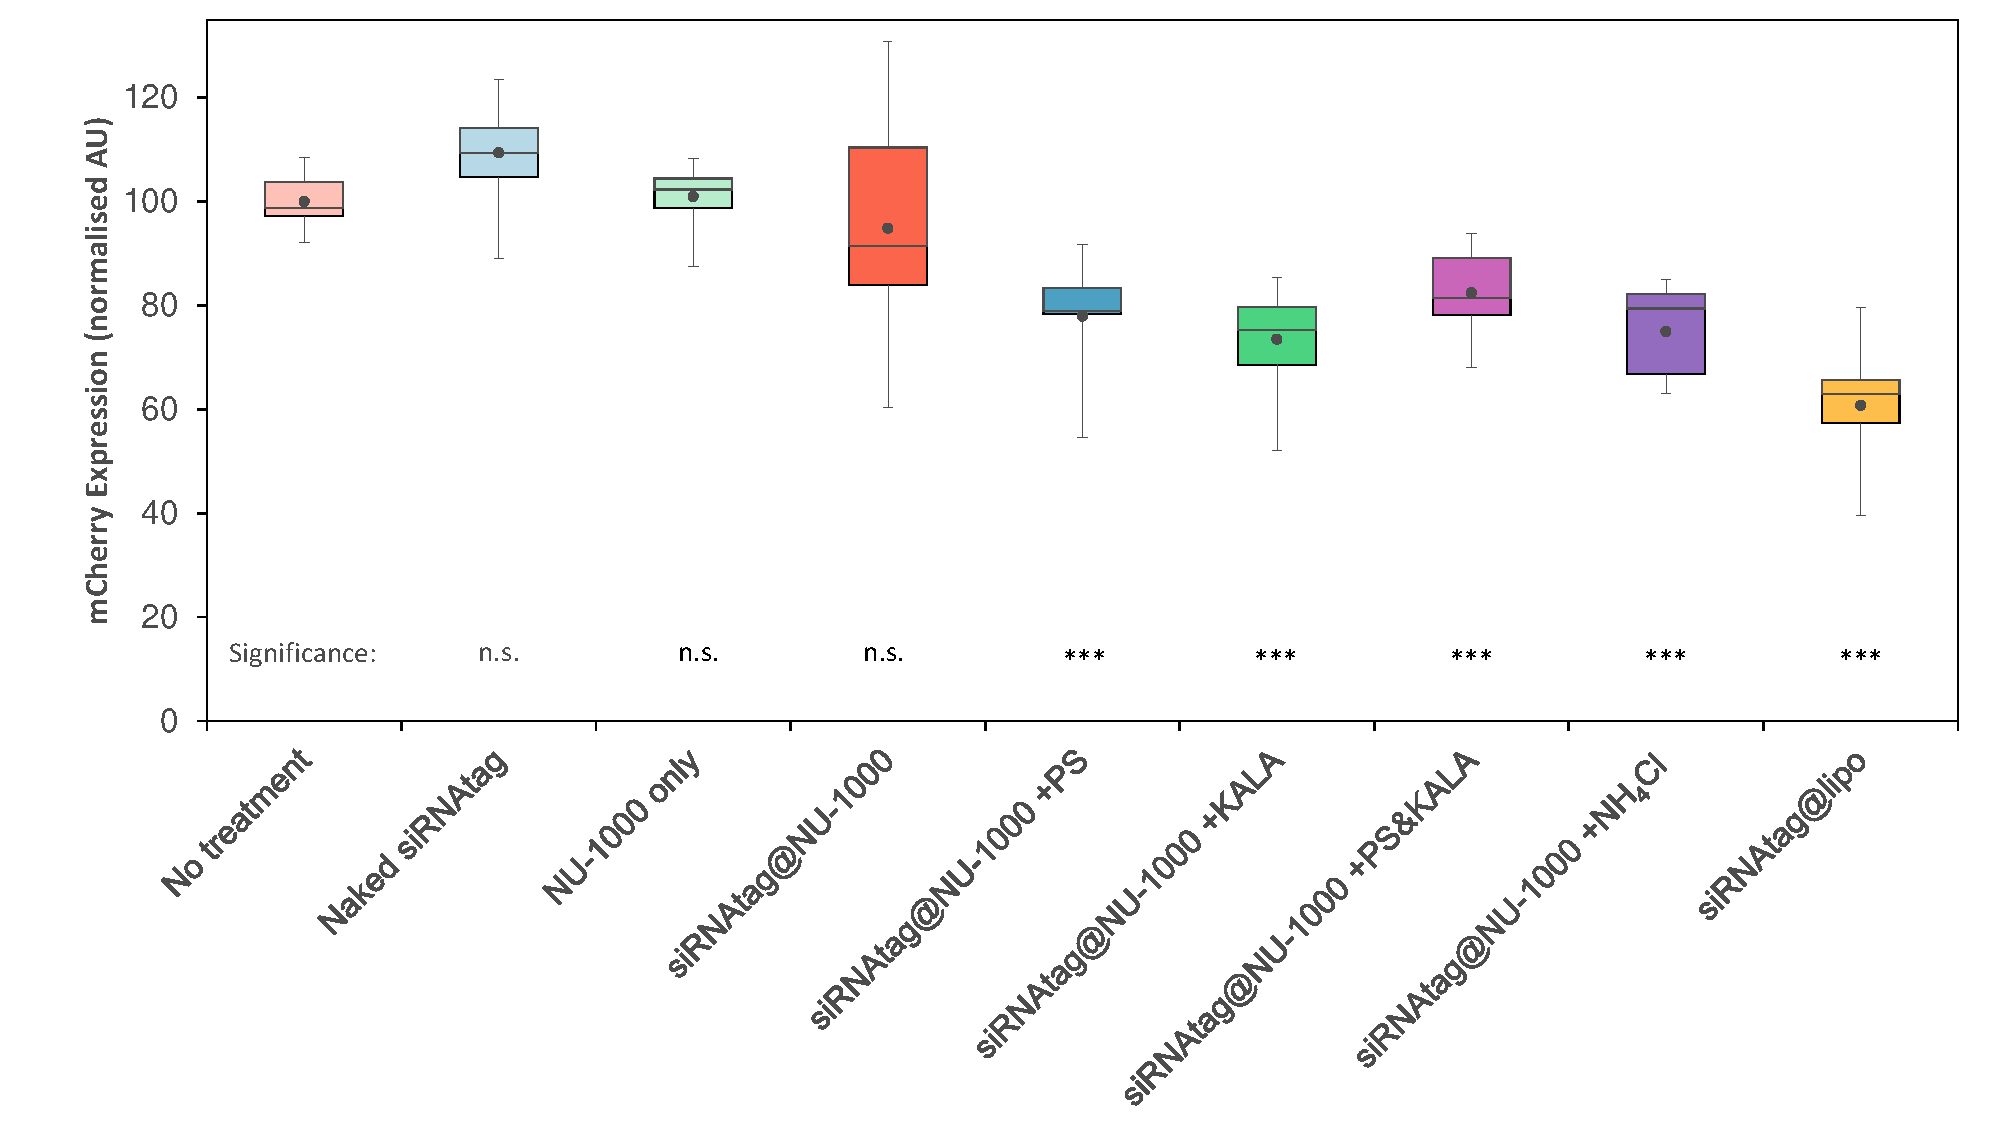
\includegraphics[width=1.0\textwidth]{mCherry-expression}
\caption[MOFs: siRNA suppresses mCherry expression when an endosome release factor is loaded to MOFs]{ Using siRNA loaded in NU-1000 causes an insignificant decrease in the mCherry expression level. Under this condition siRNA is not able to escape the endosome to cleave the mCherry. Addition of endosome release factors, such as KALA, break down the endosome, allowing the siRNA to enter the cytoplasm and perform its intended function. }
\label{fig:mCherry-expression}
\end{figure}

Three endosome release factors were used: Proton-Sponge®, an effective H\textsuperscript{+} scavenger from Sigma-Aldrich~\cite{ozkar2002nanocluster}; KALA, a cationic amphipathic cell-penetrating peptide which binds oligonucleotides and disrupts cell membrane; and ammonium chloride, which has previously been shown to induce release of molecules from sub-cellular vesicles~\cite{cervia2017distinct}. 

Figure~\ref{fig:mCherry-expression} shows that, with the addition of any release cofactor, mCherry expression level was significantly reduced. 
The expected mechanism by which the siRNA is now able to suppress mCherry experssion is as follows: siRNA and the endosome release factor load into the pores of MOFs; these MOF complexes are taken up into the cell by endocytosis, and are initially located in endosomes; the MOF starts to break down due to the endosome environment, releasing the endosome release factor and siRNA; the endosome release factor breaks down the endosome membrane before the endosome can break down the siRNA, releasing the siRNA into the cytoplasm; and finally, the siRNA can cleave mRNA, silencing expression of mCherry.
% Perhaps a few more words about the graph itself?

The proposed mechanism for the successful gene silencing is confirmed by the SIM image in Figure~\ref{fig:siRNA-MOF-uptake}d. 
In contrast to Figure~\ref{fig:siRNA-MOF-uptake}b, yellow areas show that the siRNA-MOF complex is no longer colocalised with endosomes, showing that the cofactor successfully released it from the endosome into the cytoplasm. 
Furthermore, siRNA can be seen independently in parts of the cell, as red pixels not colocalised with any other colour. 

\subsection{MOFs deliver DCA to restart the Krebs cycle, with TPP as a cofactor to target mitochondria}
As described in Section~\ref{sec:MOF-intro}, most cancers occur when cells bypass the Krebs cycle, such that mitochondria continuously divide without undergoing apoptosis~\cite{murray1993cell}.
This makes cancerous cells difficult to destroy. 
While chemotherapy techniques, such as radiation therapy, can kill the cancer cells, treatment is often non-discriminatory and destroys all cells in the area, leading to unwelcome side-effects~\cite{coates1983receiving, de1997patient, minami2010cardiovascular}. 

It has been shown DCA is able to induce apoptosis in cancer cells by restoring mitochondrial function and restarting the Krebs cycle~\cite{bonnet2007mitochondria}. 
However clinical trials so far have been unsuccessful; perhaps because of a low half-life in the body, so that a therapeutic concentration does not reach the cells. 
Loading DCA into a MOF could assist with delivery. 
In this experiment the MOF UiO-66 was used which, like the NU-1000 used in our previous MOF experiments, has a large pore size and good biocompatibility~\cite{abanades2018mechanistic}. 

Inspired by our previous work loading a cofactor with siRNA, we investigated the effect of adding a mitochondria-targeting cofactor to the MOF alongside the DCA, with the hypothesis that this would destroy more cancer cells with a lower concentration of MOF than previously shown. 
The compound triphenyl phosphonium (TPP) has been shown to assist molecules to target mitochondria, so TPP was loaded into UiO-66 MOFs as a cofactor alongside DCA. 
To obtain a thorough understanding of how the MOF complex was acting inside the cell, we used the LAG SIM to image HeLa cancer cells under different treatment conditions. 

The UiO-66 MOF used for this study was not naturally fluorescent, so was furthermore loaded with calcein to visualise it in the \SI{488}{\nano\metre} excitation channel. 
Mitochondira were labelled with MitoTracker\textsuperscript{TM} in the \SI{561}{\nano\metre} channel, and the cell nucleus was visualised with SiR-DNA in the \SI{640}{\nano\metre} channel. 

Sample SIM images are shown in Figure~\ref{fig:mito-SIM-images}. 
We confirm, with 3D reconstructions obtained by optical sectioning, that the UiO-66 MOF is successfully taken up into HeLa cells. % Should I have this as a separate figure, and highlight FPBioimage again? 
Furthermore, we can now visually observe the physical effect this treatment has on the mitochondria. 

Figure~\ref{fig:mito-30m-no-treatment} shows untreated HeLa cells with inactive mitochondria forming long, stringy projections. 
After \SI{8}{\hour} of incubation with DCA-loaded MOF, some of the mitochondria in Figure~\ref{fig:mito-8h-mof-dca} have become more circular, resembling the textbook shape of healthy mitochondria performing the Krebs cycle.
Figure~\ref{fig:mito-30m-mof-dca-tpp} shows a similar effect after just \SI{30}{\minute} when the mitochondria-targeting cofactor TPP is also loaded into the MOFs. 
After \SI{8}{\hour} of incubation with DCA and TPP both loaded into the MOF, all the mitochondria in Figure~\ref{fig:mito-8h-mof-dca-tpp} resemble the healthy textbook shape. 

To confirm this visual inspection of mitochondrial shape quantitatively, analysis was performed in Cell Profiler~\cite{carpenter2006cellprofiler}.
Image stacks of 54 cells were captured and reconstructed in two independent imaging sessions with optical-sectioning LAG SIM, and from these images \num{4811} mitochondria were extracted using the \texttt{IdentifyPrimaryObjects} plugin, as shown in Figure~\ref{cell-profiler-segmentation}. 
The ellipticity of each classified mitochondria was then calculated with the \texttt{MeasureObjectSizeShape} plugin, to produce a long list of mitochondria ellipticity under the different treatment conditions shown in Figure~\ref{fig:mito-SIM-images}. 

\begin{figure}[p]
\centering
	\begin{subfigure}[b]{0.49\textwidth}
	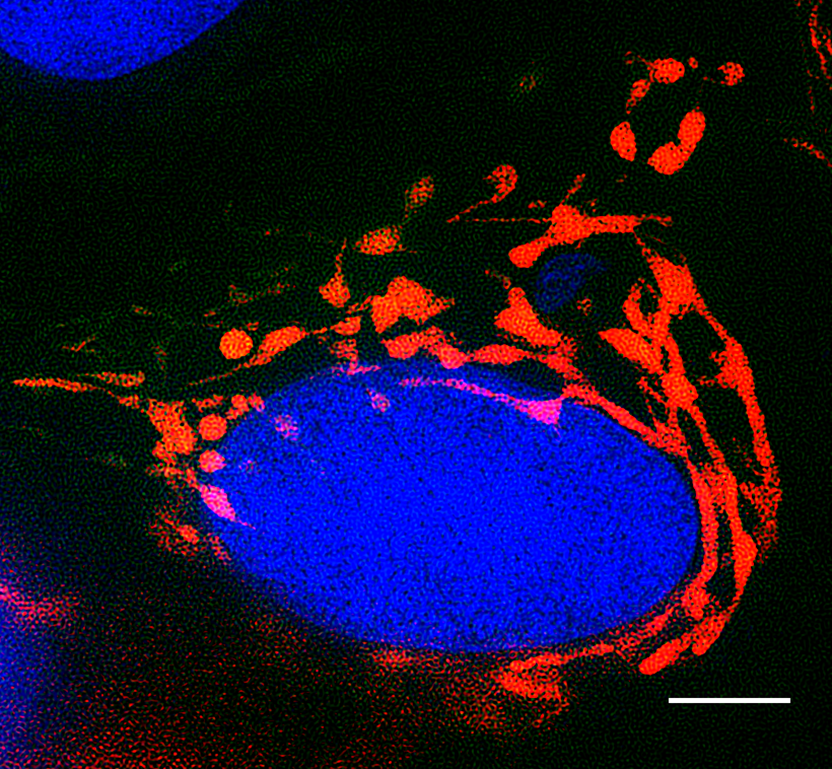
\includegraphics[width=1.0\textwidth]{mito-30m-no-treatment}
	\caption{\SI{30}{\minute}, no treatment} \label{fig:mito-30m-no-treatment}
	\end{subfigure}
	\hfill
	\begin{subfigure}[b]{0.49\textwidth}
	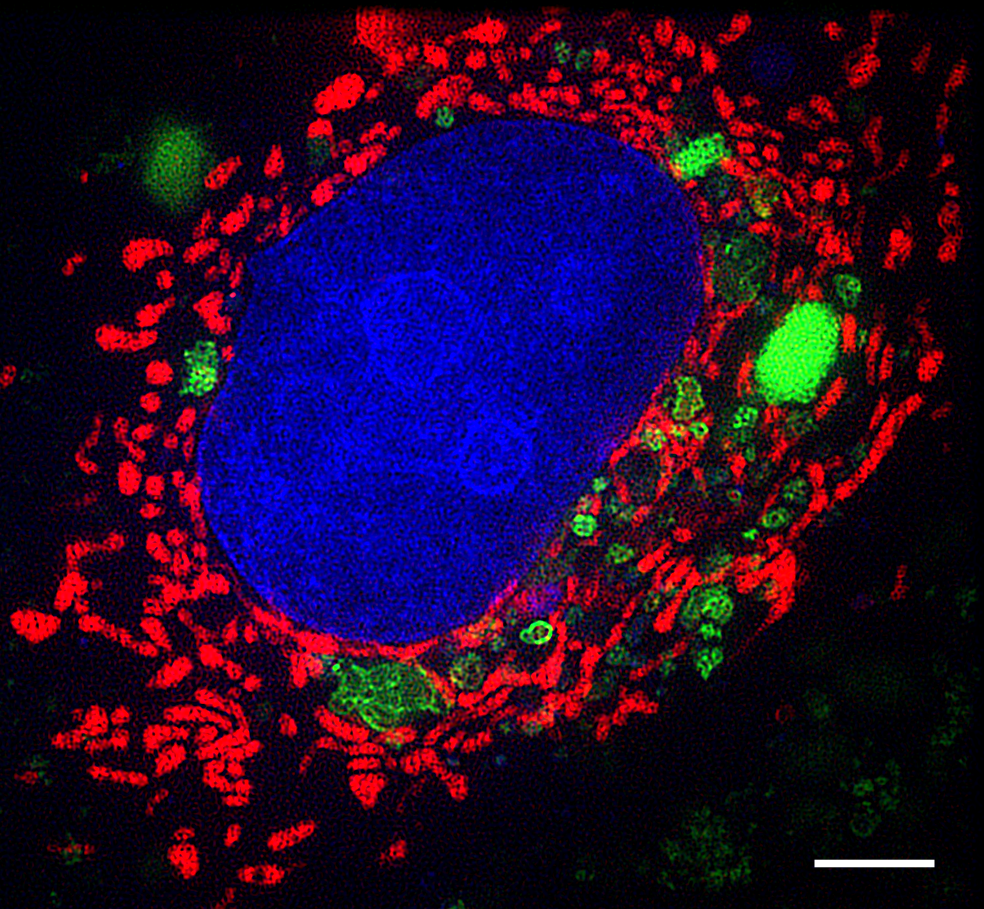
\includegraphics[width=1.0\textwidth]{mito-8h-mof-dca}
	\caption{\SI{8}{\hour}, DCA@UiO-66} \label{fig:mito-8h-mof-dca}
	\end{subfigure}
	
	~\newline
		\begin{subfigure}[b]{0.49\textwidth}
	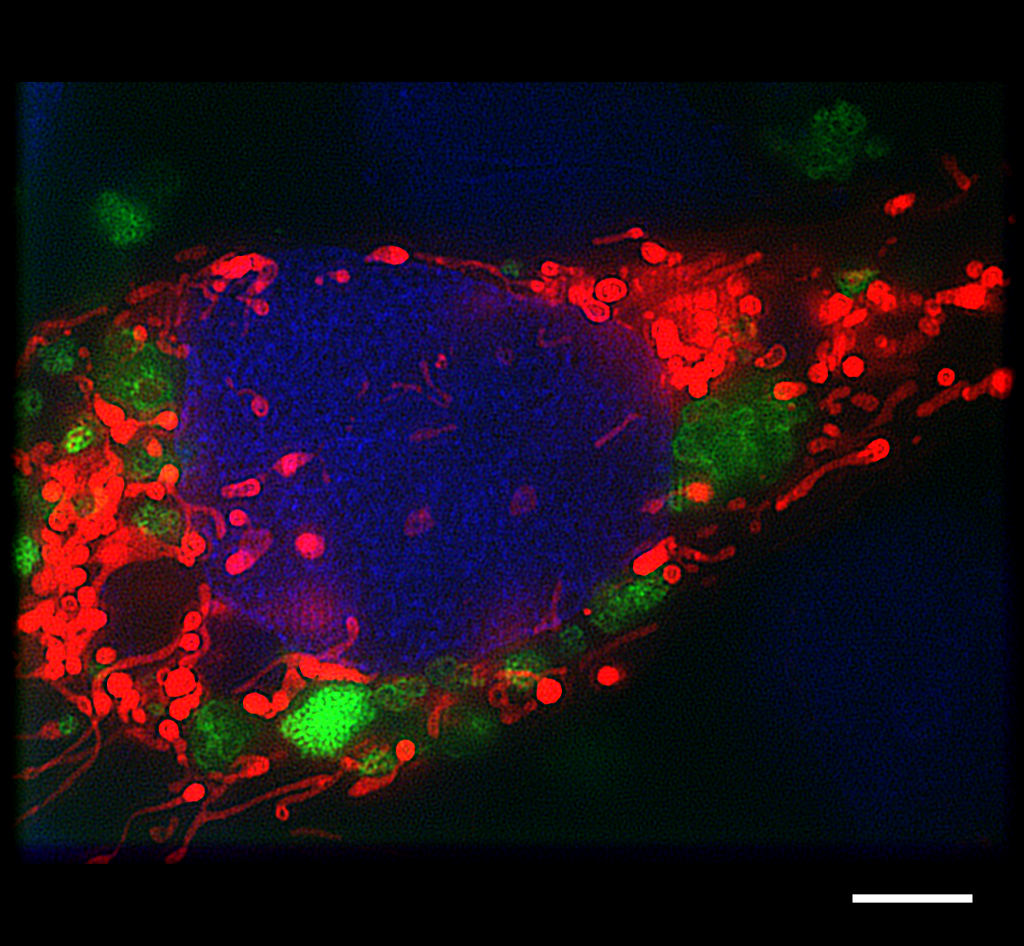
\includegraphics[width=1.0\textwidth]{mito-30m-mof-dca-tpp}
	\caption{\SI{30}{\minute}, DCA+TPP@UiO-66}\label{fig:mito-30m-mof-dca-tpp}
	\end{subfigure}
	\hfill
	\begin{subfigure}[b]{0.49\textwidth}
	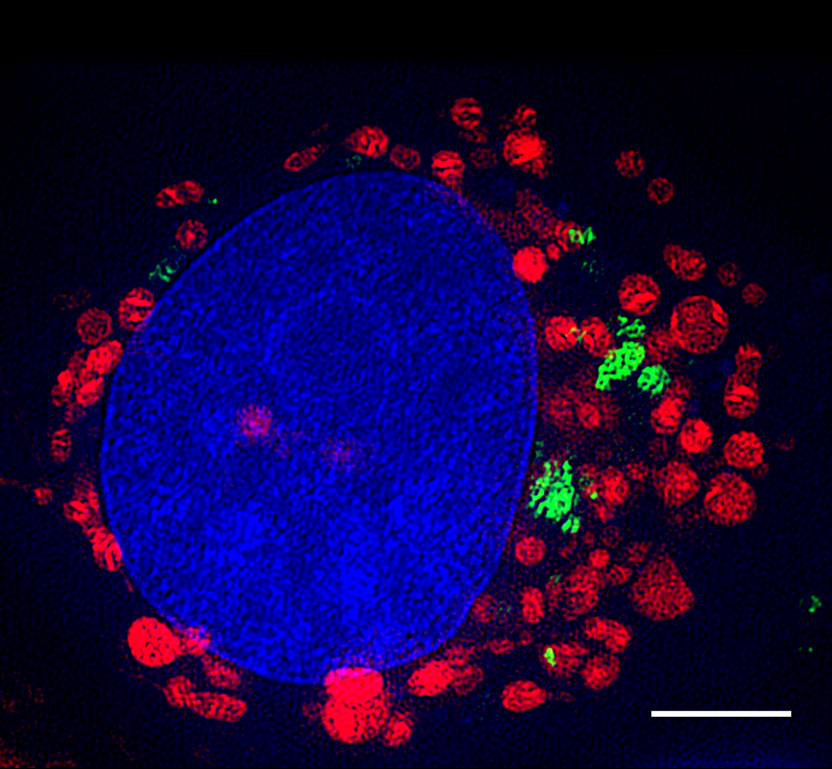
\includegraphics[width=1.0\textwidth]{mito-8h-mof-dca-tpp}
	\caption{\SI{8}{\hour}, DCA+TPP@UiO-66}\label{fig:mito-8h-mof-dca-tpp}
	\end{subfigure}
\caption[MOFs: UiO-66 MOF loaded with DCA changes mitochondria's shape]{Images show mitochondria coloured in red, MOF visible by calcein-loading coloured in green, and the nucleus labelled by SiR-DNA coloured in blue. (a) shows inactive mitochondira in untreated cells, with long stringy projections. Treating the cells with DCA-loaded UiO-66 MOF, shown in (b), causes mitochondria to lose their long, elliptical shape. (c) and (d) show that this process is enhanced by loading TPP as a cofactor, resulting in circular mitochondira after \SI{8}{\hour} of treatment. Scalebars are \SI{5}{\micro\metre}. }
\label{fig:mito-SIM-images}
\end{figure}
% Do I want a 3D projection figure too?? 
\begin{figure}[p]
\centering
	\begin{subfigure}[b]{0.49\textwidth}

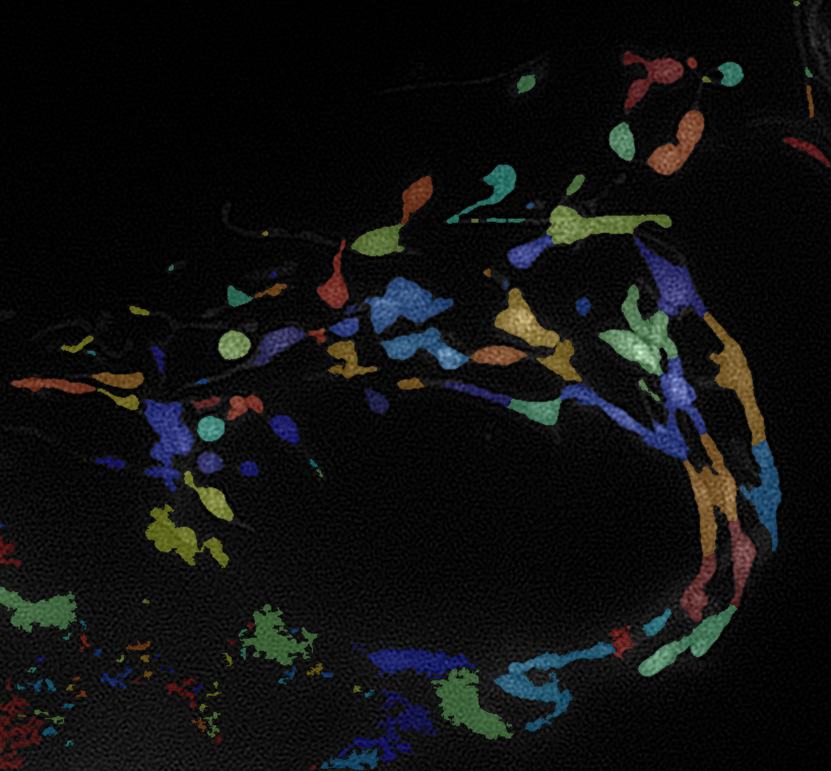
\includegraphics[width=1.0\textwidth]{mito-extract-healthy}
	\caption{}
	\end{subfigure} ~
	\begin{subfigure}[b]{0.49\textwidth}
	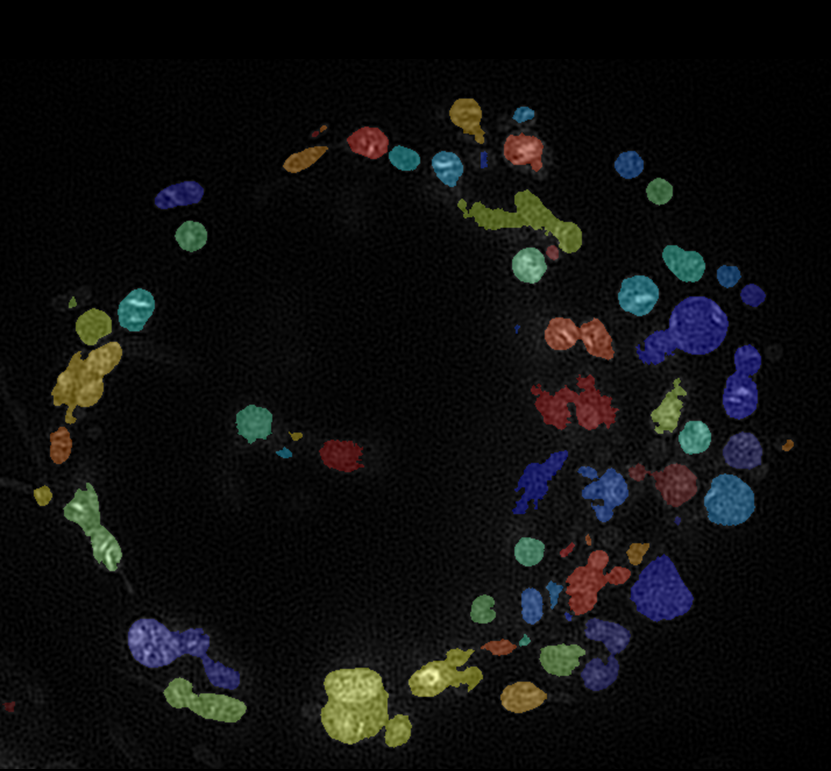
\includegraphics[width=1.0\textwidth]{mito-extract-unhealthy}
	\caption{}
	\end{subfigure}
\caption[MOFs: Mitochondria segmentation in Cell Profiler allow statistical shape analysis]{The Cell Profiler\cite{carpenter2006cellprofiler} protocol identifies and segments mitochondria in the cell, shown here applied to Figures~\ref{fig:mito-30m-no-treatment} and~\ref{fig:mito-8h-mof-dca-tpp}. The ellipticity of segments is calculated to provide statistics about the change in mitochondria shape caused by DCA-loaded UiO-66. Scalebars are \SI{5}{\micro\metre}. }
\label{fig:cell-profiler-segmentation}
\end{figure}

The mitochondria ellipticity statistics were analysed with a one-way ANOVA test in Graphpad Prism~\cite{graphpadprism}, and the results are presented in Figure~\ref{fig:mito-ellipticity-graph}. 
Adding DCA-loaded MOF causes a decrease in ellipticity, however there is not a statistically significant difference between the mean ellipticities, with $p=0.2083$. 
With TPP also added to the MOF as a cofactor, a $p=0.0194$ significant decrease in the ellipticity of mitochondria is observed. 
Furthermore after \SI{8}{\hour} of treatment there is a significant decreases between the DCA+TPP MOFs and the DCA-only MOFs. 
These statistics support the visual inspection of Figure~\ref{fig:mito-SIM-images}. 

Furthermore, these findings corroborate data from FACS measurements shown in Figure~\ref{fig:dca-tpp-cytotoxicity}. 
The graphs show that MOFs loaded with both DCA and TPP are more effective at inducing cell death than MOFs with DCA alone, measured by the MTS assay~\cite{mosmann1983rapid, mtsassay}. 
Moreover, the graphs show that this enables a lower concentration of drug to be administered for the same therapeutic effect.

\begin{figure}[htbp!]
\centering
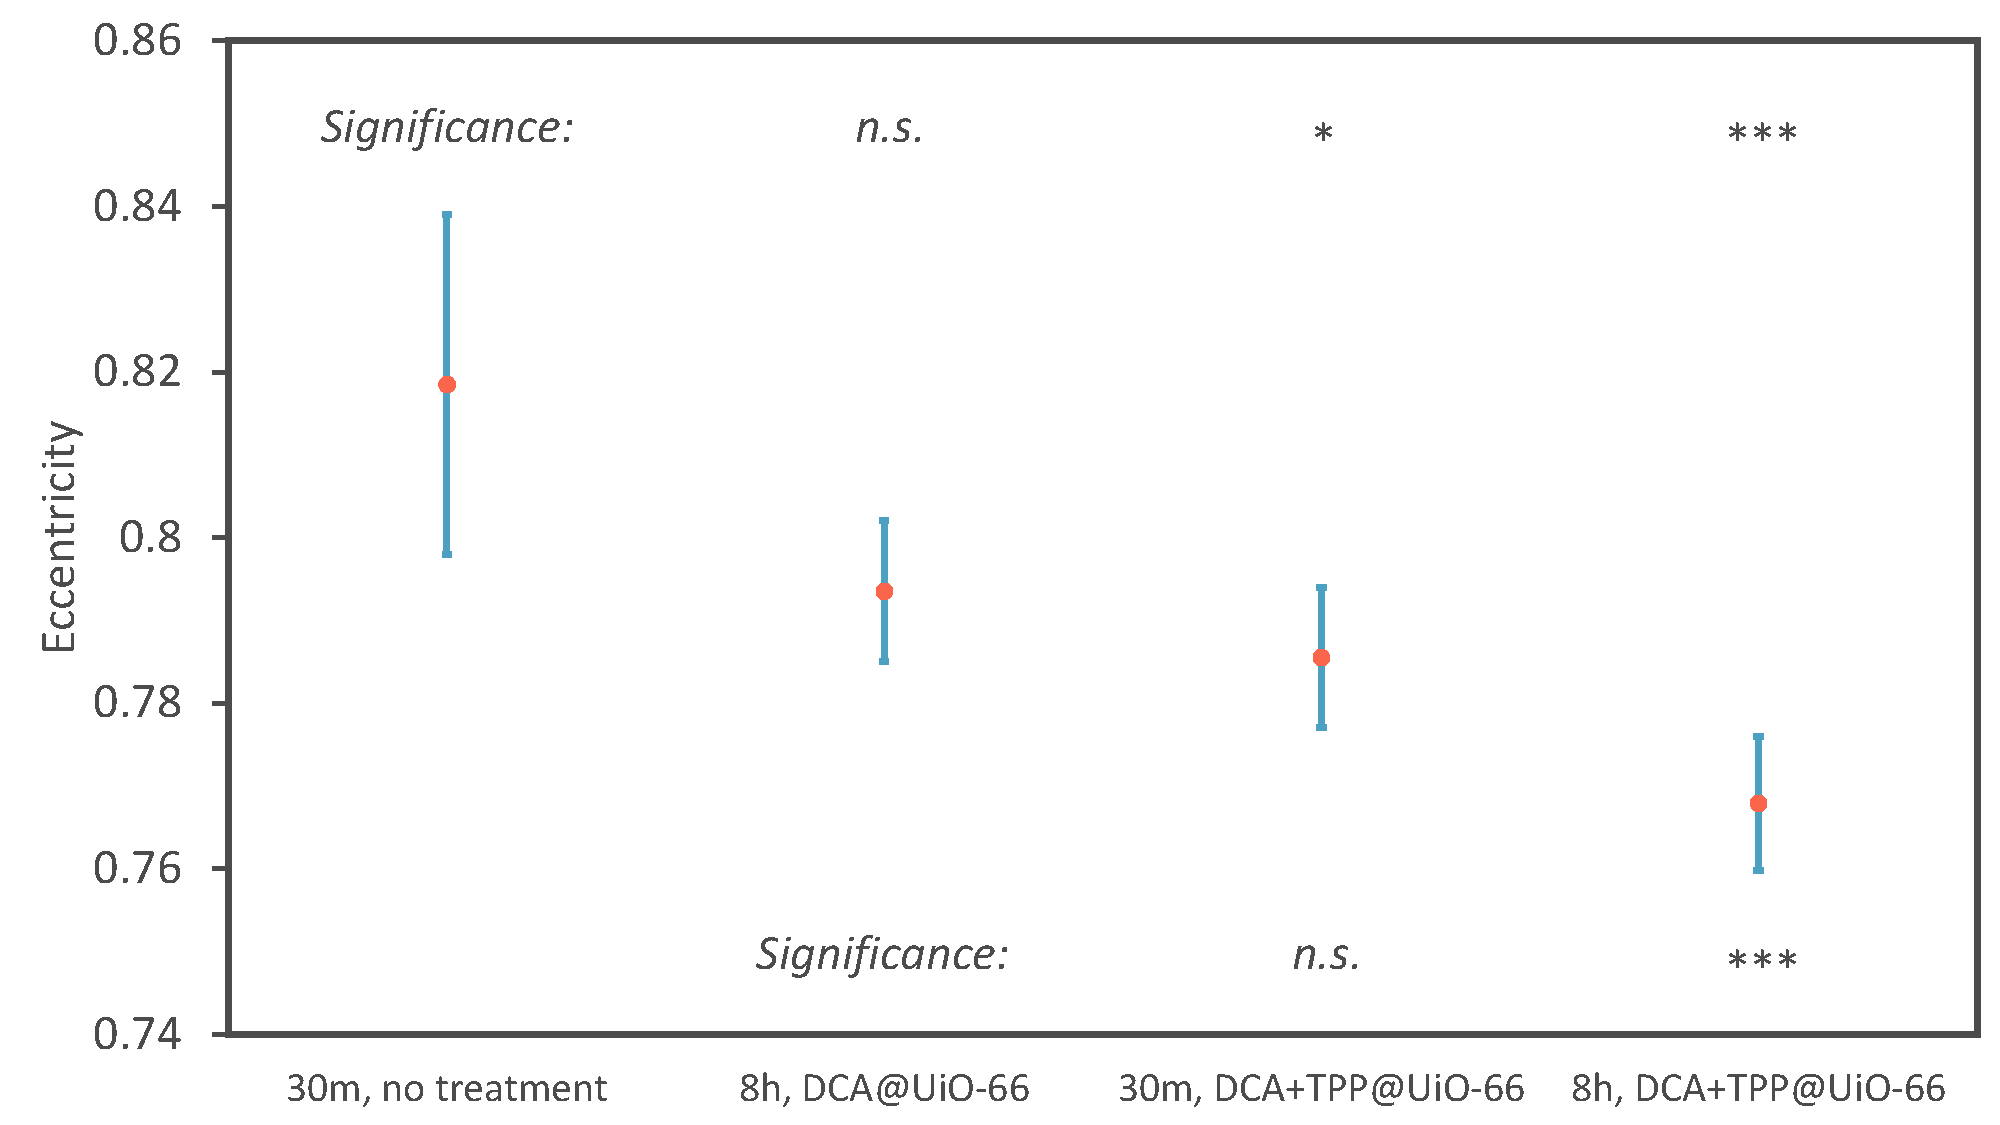
\includegraphics[width=1.0\textwidth]{mito-ellipticity-graph}
\caption[MOFs: Mitochondria become more circular when treated with ] {Mitochondria are affected by the DCA-UiO-66 treatment, making them more circular in shape. The reduction in eccentricity is not significant without addition of TPP as a mitochondira-targetting cofactor. $*: p<0.05$, $***: p<0.001$} 
\label{fig:mito-ellipticity-graph}
\end{figure}

\begin{figure}[htbp!]
\centering
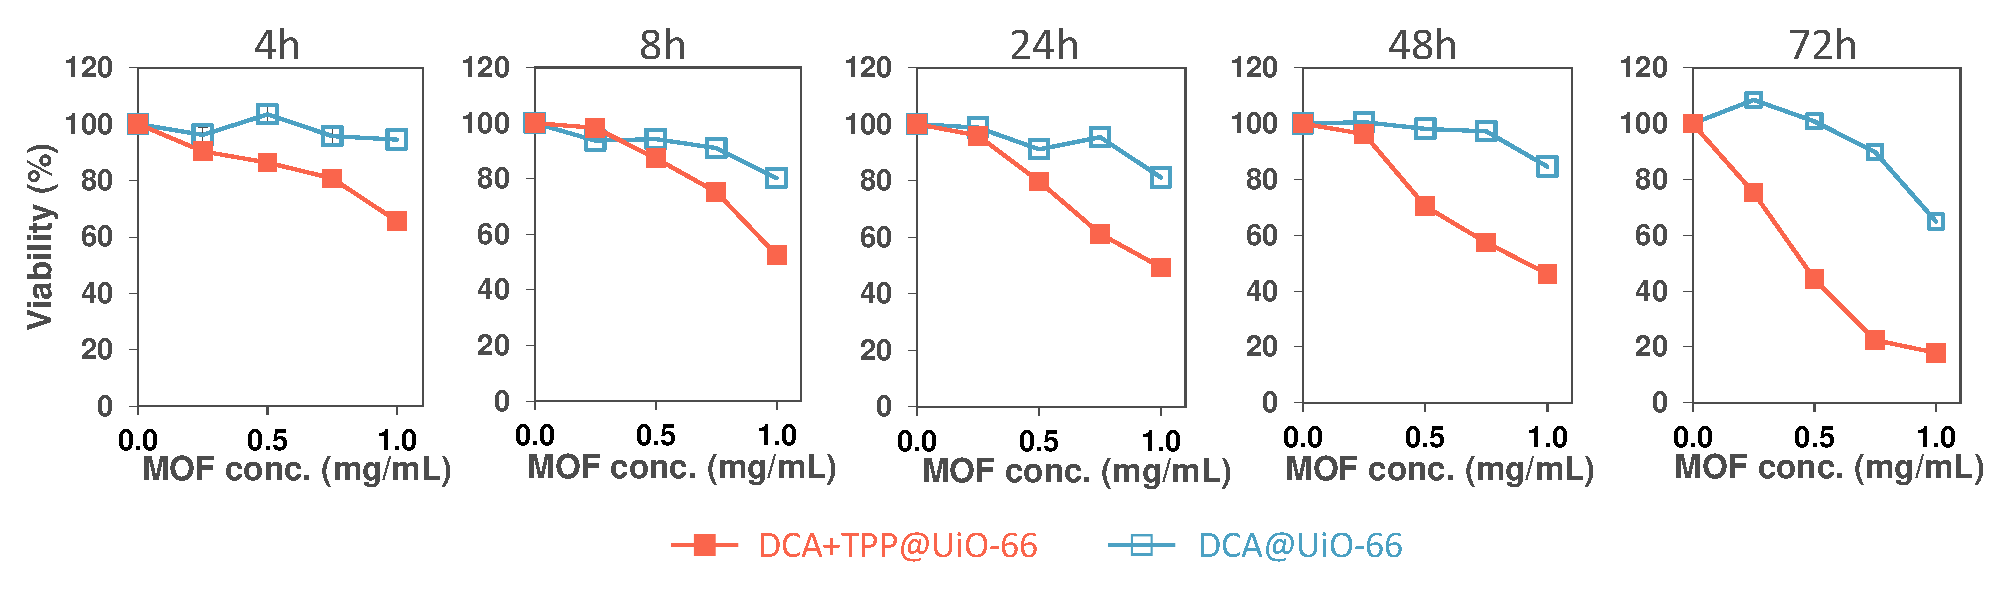
\includegraphics[width=1.0\textwidth]{dca-tpp-cytotoxicity}
\caption[MOFs: Loading MOFs with TPP as a cofactor facilitates lower drug concentration] {A cytotoxicity study corroborates observations of microscopy images that MOFs loaded with TPP as a cofactor are more effective at inducing cell death in cancerous HeLa cells than MOF loaded with DCA alone. This allows treatment with lower concentrations of drug for the same therapeutic effect.} 
\label{fig:dca-tpp-cytotoxicity}
\end{figure}


\section{Conclusion} \label{sec:mof-conclusion}
The three experiments presented in this chapter utilise MOFs as a drug delivery vehicle for cancer treatment. 
We have shown through a variety of techniques that MOFs can be successfully loaded with therapeutic molecules which would otherwise be degraded in extra-cellular space, and subsequently can delivery these drugs to the cell. 

Furthermore, we have observed a significant decrease in cancer cell viability when MOFs are used as a delivery vehicle. 
Two techniques, based on delivering siRNA for gene silencing and DCA for mitochondrial degradation which restarts the Krebs' cycle, have emerged as successful treatment strategies on cancerous HeLa cells. 
Concerns regarding the burst release effect, where much of the MOF's therapeutic payload is released before the MOF has entered the cell, have been addressed with a temperature treatment strategy which induces pore collapse to delay release. 

The utilisation of optical sectioning provided by the LAG SIM has allowed both visual confirmation of biological hypotheses and large datasets for statistical analysis. 

Throughout the chapter, 3D reconstructions have shown that MOF is able to pass the cell membrane and enter cells; an endocytosis study showed that this occurs through the clathrin-mediated pathway. 
Inside the cells, MOFs are colocalised with endosomes; this can prevent the MOF's payload having a therapeutic effect without addition of an endosome release factor. 
When Proton-Sponge®, KALA or NH\textsubscript{4}Cl were loaded into the MOF as cofactors, a significant decrease in cell viability was measured, and furthermore SIM images confirmed that MOF was no longer colocalised with endosomes. 

LAG SIM's fast imaging speed allows a large number of cells to be imaged in a single session. 
This firstly has the advantage that cells do not spend long on the microscope stage, where non-optimal conditions can cause apoptosis[check] of cells; but rather cells can be left in the incubator for most of a 24-hour time course study. 
Secondly, meaningful statistics can be gathered when a large number of cells are imaged, allowing visual observations to be rendered as statistically significant results.

Overall this chapter has demonstrated the LAG SIM's capability for facilitating hypothesis-driven research supporting and confirming measurements from other techniques and providing visualisation to develop pioneering treatments in the fight against cancer. 

\section{Future work}
Using MOFs as a drug delivery vehicle has been demonstrated as an effective treatment for cultured HEK-293 cells. 
The next step towards developing a drug that can be used to treat humans is to assess the treatment on a model organism. 
Work is now underway to apply the siRNA-MOF treatment to mice, to observe the effectiveness of the therapy at organism level and assess any toxicity issues. 

This chapter has presented just 3 MOFs, NU-901, NU-1000, and UiO-66, which have desirable properties for use as a drug delivery vehicle. 
However our previous work~\cite{moghadam2018computer} has shown that due to the tens-of-thousands of MOF structures possible, selecting the perfect MOF is non-trivial. 
We have previously built an online tool for screening a database of drugs to select the one most-suited to a given application. 
Though the tool, accessible at \url{https://aam.ceb.cam.ac.uk/mof-explorer/}, is currently set up for optimising gas storage solutions, adding biologically relevant axes such as toxicity and payload release time could reveal an even better MOF than those already investigated. 